\documentclass[letterpaper,12pt]{report}
\usepackage[spanish]{babel}
\usepackage[utf8]{inputenc}
\usepackage{graphicx}
\usepackage{amsfonts,amsmath,color,amssymb,float, amsthm,mathrsfs}  
\usepackage[right=3cm,left=2cm,top=2cm,bottom=2cm,headsep=0.7cm,footskip=0.5cm]{geometry}
\usepackage{enumerate}
\usepackage{wrapfig} 
\usepackage[rflt]{floatflt} 
\usepackage{framed}
\usepackage[most]{tcolorbox}
\usepackage{xcolor} 
\colorlet{shadecolor}{green!20}
\setlength\FrameSep{0.5ex}
\usepackage{thmtools}
\usepackage{esint}
\usepackage{cancel}
\usepackage{listings} 
\usepackage{pstricks, caption}
\usepackage[colorlinks]{hyperref}
\usepackage{csquotes}
\usepackage{fullpage}
\usepackage{enumitem}
\usepackage{etoolbox}
\usepackage{tcolorbox}
\usepackage{tikz}
\usetikzlibrary{arrows,babel}


\decimalpoint
\newcommand{\grad}{^\circ}
\newlength{\drop}
\DeclareMathOperator{\sign}{sgn}
\DeclareMathOperator{\Log}{Log}
\providecommand{\norm}[1]{\lVert#1\rVert}

%%%%%%%%%Entornos: Teoremas, Defs,etc%%%%%%%
\theoremstyle{definition}

\newtheorem{defis}{Definiciones}[section]
\newtheorem{corolario}{Corolario}[section] 
\newtheorem{lema}{Lema}[section] 

\newtheorem{protoexample}{Ejemplo}[section]
\newenvironment{ejemplo}
   {\colorlet{shadecolor}{orange!15}\begin{shaded}\begin{protoexample}}
   {\end{protoexample}\end{shaded}}

\newtheorem*{protoproof}{Demostración}
\newenvironment{demo}
   {\colorlet{shadecolor}{blue!10}\begin{shaded}\begin{protoproof}}
   {\end{protoproof}\end{shaded}}

\newenvironment{Rdbleftbar}{%
  \def\FrameCommand{\textcolor{red}{\vrule width0.6pt}\hspace{0.15em}\textcolor{red}{\vrule width0.6pt} \hspace{0.5em}}%
  \MakeFramed {\advance\hsize-\width \FrameRestore}}%
 {\endMakeFramed}

 \newenvironment{Bdbleftbar}{%
  \def\FrameCommand{\vrule width0.6pt\hspace{0.15em}\vrule width0.6pt \hspace{0.5em}}%
  \MakeFramed {\advance\hsize-\width \FrameRestore}}%
 {\endMakeFramed}

\newenvironment{Gdbleftbar}{%
  \def\FrameCommand{\textcolor{green}{\vrule width0.6pt}\hspace{0.15em}\textcolor{green}{\vrule width0.6pt} \hspace{0.5em}}%
  \MakeFramed {\advance\hsize-\width \FrameRestore}}%
 {\endMakeFramed}
 
% With parskip

\usepackage[indent=0.6cm]{parskip}

\declaretheorem[%
name            =Teorema,%
numberwithin=section,
postheadhook    =\vspace*{\parskip} \begin{Rdbleftbar}\vspace*{-5pt},%
prefoothook     =\vspace*{-1pt}\end{Rdbleftbar}%
]{teorema}

\declaretheorem[%
name            =Definición,%
numberwithin=section,
postheadhook    =\vspace*{\parskip}\begin{Bdbleftbar}\vspace*{-5pt},%
prefoothook     =\vspace*{-1pt}\end{Bdbleftbar}%
]{defi}

\declaretheorem[%
name            = Proposición,%
numberwithin=section,
postheadhook    =\vspace*{\parskip}\begin{Gdbleftbar}\vspace*{-5pt},%
prefoothook     =\vspace*{-1pt}\end{Gdbleftbar}%
]{propo}   
%%%%%%%%%%%%%%%%%%%%%%%%%%%%%%%%%%%%%%%%%%%%%%

%%%%%%%%%%%%Fancy Chapters%%%%%%%%%%%%%%%%%
%Options: Sonny, Lenny, Glenn, Conny, Rejne, Bjarne, Bjornstrup
\usepackage[Lenny]{fncychap}
%%%%%%%%%%%%%%%%%%%%%%%%%%%%%%%%%%%%%%%%%%%

%Referencias
\usepackage[backend=biber]{biblatex}
\addbibresource{Referencias.bib}

\begin{document}

\begin{titlepage}
 \drop=0.1\textheight
    \centering
    \vspace*{\baselineskip}
    \rule{\textwidth}{1.6pt}\vspace*{-\baselineskip}\vspace*{2pt}
    \rule{\textwidth}{0.4pt}\\[\baselineskip]
    {\scshape\Huge Física matemática} \\[0.2\baselineskip]
    \rule{\textwidth}{0.4pt}\vspace*{-\baselineskip}\vspace{3.2pt}
    \rule{\textwidth}{1.6pt}\\[\baselineskip]
    {\Large Autor: \par}
{\Large Alejandro Saavedra \par}
\vfill
{\large Diciembre 2022 \par}
{\large v1.0 \par}
\end{titlepage}

\tableofcontents

\chapter{Espacio de funciones}

\section{Definiciones}

\begin{defi}
Denotemos por $\mathcal{C}_0 [a,b]$ al conjunto de funciones complejas continuas de una variable real $t \in [a,b]$.
\end{defi}

Notemos que claramente se cumple:
\begin{shaded}
$$\mbox{si} ~ f,g \in \mathcal{C}_0[a,b] ~\Rightarrow~ f + g \in \mathcal{C}_0 [a,b]$$
\end{shaded}

y 
\begin{shaded}
$$\mbox{si} ~ f \in \mathcal{C}_0[a,b] ~\mbox{y}~ \lambda \in \mathbb{C} ~\Rightarrow~ \lambda f \in  \mathcal{C}_0[a,b].$$ 
\end{shaded}

\begin{defi}
Una función $f: [a,b] \longrightarrow \mathbb{C}$ es \textbf{seccionalmente continua} si $[a,b]$ tiene una partición finita $a = t_0 < t_1 < \cdots < t_n = b$ tal que $f$ es continua y acotada en cada intervalo abierto $]t_i, t_{i+1}[, i = 0, \dots, n-1$.

Denotaremos por $\mathcal{C}[a,b]$ al conjunto de funciones complejas seccionalmente continuas.
\end{defi}

Geométricamente, $f: [a,b] \longrightarrow \mathbb{C}$ es una curva en el plano complejo y la condición de seccionalmente continua se puede apreciar en la figura \ref{fig:FunciónSC}. 

\begin{figure}
    \centering
    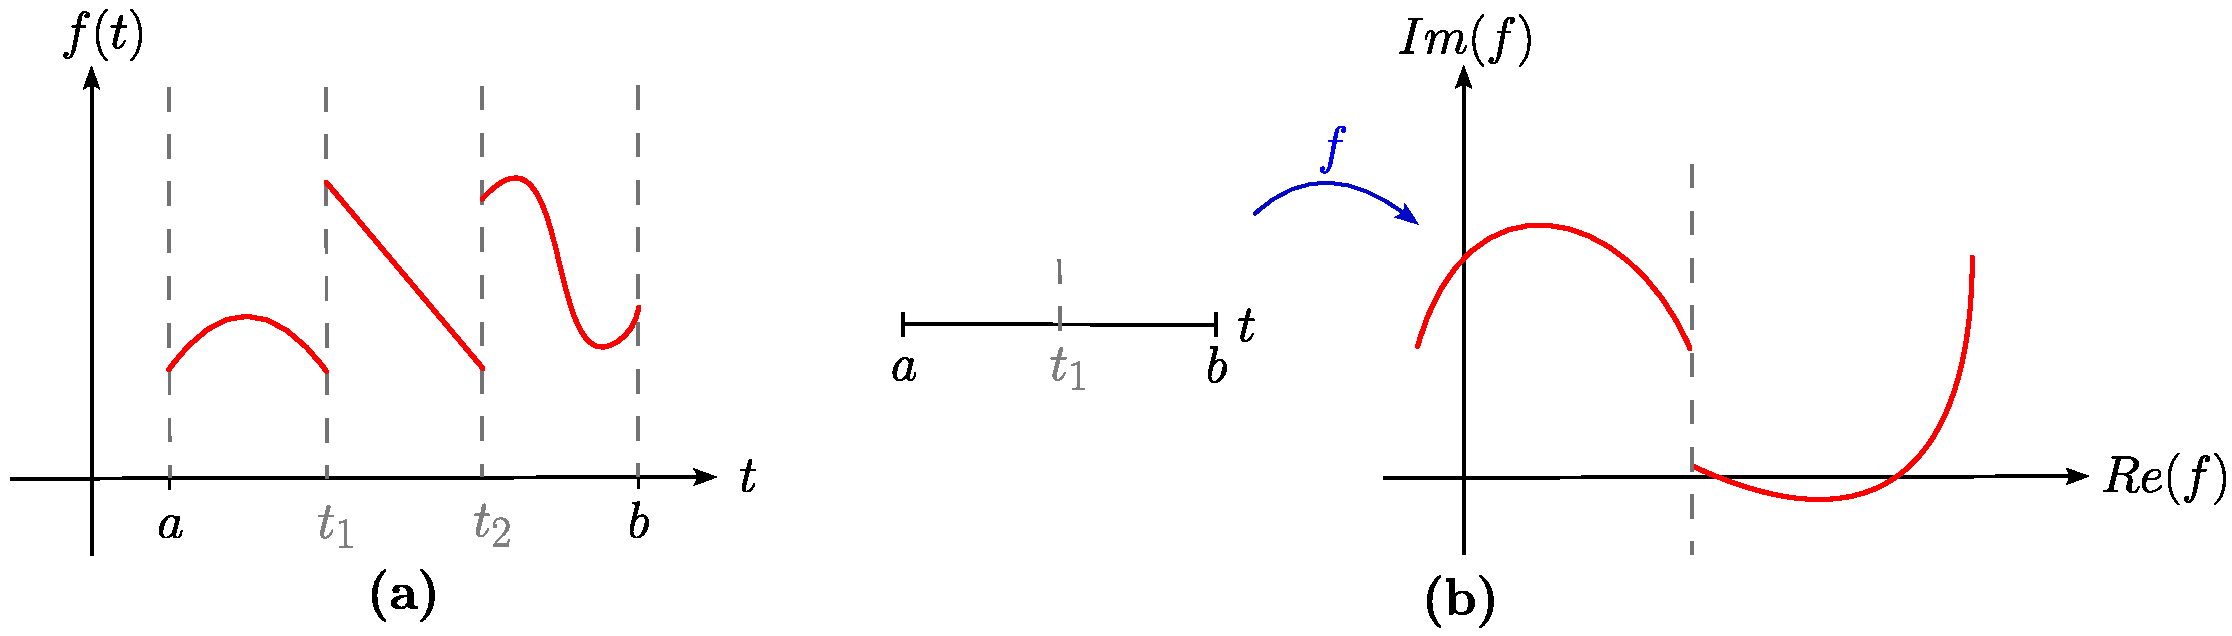
\includegraphics[scale=0.45]{Figuras/FuncionSC.pdf}
    \caption{En (a) una función de la forma $f: [a,b] \rightarrow \mathbb{R}$ y en (b) una función de la forma $f: [a,b] \rightarrow \mathbb{C}$, ambas seccionalmente continuas.}
    \label{fig:FunciónSC}
\end{figure}

Podemos afirmar que los conjuntos $\mathcal{C}_0 [a,b]$ y $\mathcal{C}[a,b]$ forman espacios vectoriales sobre el cuerpo de los complejos. Además, $\mathcal{C}_0 [a,b] \subset \mathcal{C} [a,b].$

\begin{defi}
Consideremos dos funciones $f,g \in \mathcal{C}[a,b]$. Definimos su \textbf{producto escalar} como
$$\boxed{\langle f , g \rangle = \int_a^b f(t) g^*(t) \,dt }$$
\end{defi}

\begin{propo}[Propiedades del producto escalar] \label{ProductoEscalar}
 Sean $f,g,h \in \mathcal{C}[a,b]$ y  $\lambda \in \mathbb{C}$.
 
 \begin{itemize}
     \item $\langle f , g \rangle = \langle g, f \rangle^*$
     \item $\langle f , g + h \rangle = \langle f , g \rangle + \langle f , h \rangle$
     \item $\langle f + g , h \rangle = \langle f , h \rangle + \langle g , h \rangle$
     \item $\langle \lambda f , g \rangle = \lambda \langle f , g \rangle$
     \item $\langle  f , \lambda g \rangle = \lambda^*\langle f , g \rangle$
     \item Si $f \not\equiv 0$, entonces $\langle f , f \rangle > 0$
 \end{itemize}
\end{propo}

\textbf{Observación:} Con respecto a la última propiedad, se tiene que 
$$\langle f , f \rangle = \int_a^b |f(t)|^2 \,dt = 0 ~\mbox{NO IMPLICA}~ f = 0.$$

Por esto se define la relación de equivalencia \footnote{$m(E) = 0$ denota que $E$ es un conjunto de medida cero.}
$$f = g ~ c.t.p ~\Leftrightarrow~ f(t) = g(t), \forall t \in [a,b]-E, \mbox{con}~ m(E) = 0.$$

Esta relación se expresa diciendo que $f = g $ casi en todas partes.

\textbf{Notación:} $f \equiv g ~\Leftrightarrow~ f = g ~c.t.p$

Esencialmente una relación de equivalencia es una relación de igualdad, bajo la cual dos funciones equivalentes se consideran ``iguales". Así, toda función $f = 0 ~c.t.p$, o simplemente $f\equiv 0$, se considera como la función nula.

\begin{defi}
Un espacio vectorial complejo dotado de un producto escalar con las propiedades de la proposición \ref{ProductoEscalar}, se conoce como \textbf{espacio pre-Hilbert}.
\end{defi} 

\begin{defi}
Sea $f \in \mathcal{C}[a,b]$. Definimos su \textbf{norma} como
$$\norm{f} = \sqrt{\langle f,f \rangle} \in \mathbb{R}.$$
\end{defi}

\begin{propo}
Sean $f,g \in \mathcal{C}[a,b]$ y $\lambda \in \mathbb{C}$.

\begin{itemize}
    \item $\norm{f} \geq 0$
    \item $\norm{\lambda f} = |\lambda| \norm{f}$
    \item $|\langle f| g \rangle | \leq \norm{f} \cdot \norm{g}$ (Desigualdad de Cauchy-Schwarz)
    \item $\norm{f \pm g} \leq \norm{f} + \norm{g}$ (Desigualdad triangular)
    \item Si $f \not\equiv 0$, entonces $\norm{f} > 0$.
\end{itemize}
\end{propo}

\begin{demo}
Demostraremos solo la desigualdad de Cauchy-Schwarz y la triangular.

\begin{itemize}
    \item \textbf{Desigualdad de Cauchy-Schwarz}:
    
    Sea $\lambda \in \mathbb{C}$ arbitrario,
\begin{align*}
0 \leq \norm{\lambda f + g}^2 = \langle \lambda f + g , \lambda f + g\rangle &= \langle \lambda f , \lambda f \rangle + \langle \lambda f , g \rangle + \langle g, \lambda f \rangle + \langle g , g \rangle \\
&= \lambda \lambda^* \norm{f}^2 + \lambda \langle f,g\rangle + \lambda^* \langle g,f\rangle + \norm{g}^2.
\end{align*}

Siendo $\lambda$ arbitrario, consideremos entonces
\begin{equation*}
    \lambda = - \frac{\langle g,f \rangle}{\norm{f}^2} ~\Rightarrow~ \lambda^* = - \frac{\langle f,g\rangle}{\norm{f}^2}, \quad \norm{f} \neq 0.
\end{equation*}

Luego, 
$$0 \leq \frac{|\langle f, g \rangle|^2}{\norm{f}^4} \norm{f}^2 - 2 \frac{|\langle f,g \rangle|^2}{\norm{f}^2} + \norm{g}^2 = -\frac{|\langle f,g \rangle|^2}{\norm{f}^2} + \norm{g}^2. $$

Lo que implica 
$$|\langle f,g \rangle|^2 \leq \norm{f}^2 \cdot \norm{g}^2 ~\Rightarrow~ \boxed{|\langle f , g \rangle| \leq \norm{f} \cdot \norm{g}}$$

Si suponemos que $\norm{f} = 0$, $f \equiv 0$ y la desigualdad se demuestra trivialmente.

 \item \textbf{Desigualdad triangular}: De la definición de norma
 \begin{align*}
     \norm{f\pm g}^2 = \langle  f \pm g , f \pm g \rangle &= \langle f \pm g , f \rangle \pm \langle f \pm g , g\rangle \\
     &= \langle f,f \rangle \pm \langle f , g \rangle^* \pm \langle f,g \rangle +  \langle g,g \rangle \\
     &= \norm{f}^2 \pm 2 Re(\langle f,g \rangle) + \norm{g}^2.
 \end{align*}
 
 Como $\pm Re(z) \leq |z|$ para todo $z \in \mathbb{C}$, obtenemos que 
 $$\norm{f\pm g}^2 \leq \norm{f}^2+ 2 |\langle f,g \rangle| + \norm{g}^2.$$
 
 Por la desigualdad de  Cauchy-Shwarz:
 $$\norm{f\pm g}^2 \leq \norm{f}^2 + 2 \norm{f} \cdot \norm{g} + \norm{g}^2 = (\norm{f} + \norm{g})^2 ~\Rightarrow~ \boxed{\norm{f \pm g} \leq \norm{f} + \norm{g}}$$
\end{itemize}


\end{demo}

\section{Sucesiones y series de funciones}

\begin{defi}[Sucesión de funciones]
Sea $\{f_n\}_{n \in \mathbb{N}}$ una sucesión de funciones 
$$f_n: D \subseteq \mathbb{R} \longrightarrow \mathbb{C}.$$

y considere $f: D \subseteq \mathbb{R} \longrightarrow \mathbb{C}$.

\begin{enumerate}
    \item Diremos que $\{f_n\}_{n \in \mathbb{N}}$ \textbf{converge puntualmente} a $f$ si dado $t \in D$ se tiene que la sucesión de números complejos $\{f_n(t)\}_{n \in \mathbb{N}}$ converge a $f(t)$ donde $f$ se llama la \textbf{función límite} de $\{f_n\}_{n \in \mathbb{N}}$, matemáticamente:
    $$(\forall t \in D)(\forall \varepsilon > 0)(\exists N(t,\varepsilon) \in \mathbb{N})(n \geq N ~\Rightarrow~ |f_n(t) - f(t)| < \varepsilon).$$
    
    \textbf{Notación:} $\lim\limits_{n \to + \infty} f_n(t) = f(t)$.
    
    \item  Diremos que $\{f_n\}_{n \in \mathbb{N}}$ \textbf{converge uniformemente} a $f$ si 
     $$(\forall \varepsilon > 0)(\exists N(\varepsilon) \in \mathbb{N})(n \geq N ~\wedge~ \forall t \in D ~\Rightarrow~ |f_n(t) - f(t)| < \varepsilon).$$
     
     \textbf{Notación:} $\lim\limits_{n \to + \infty} f_n(t) = f(t) ~[uniforme]$.
\end{enumerate}

\end{defi}

\textbf{Observación:} Es fácil de ver que si $\{f_n\}_{n\in \mathbb{N}}$ converge uniformemente a $f$, entonces $\{f_n\}_{n\in \mathbb{N}}$ converge puntualmente a $f$.

\begin{defi}[Serie de funciones]
Sea $\{f_n\}_{n \in \mathbb{N}}$ una sucesión de funciones
$$f_n: D \subseteq \mathbb{R} \longrightarrow \mathbb{C}.$$

Sea $F_n = \sum\limits_{k=1}^n f_k$. Se llama \textbf{serie de funciones} a la sucesión de sumas parciales $\{F_n\}_{n\in\mathbb{N}}$ y se denota por $\sum\limits_{n=1}^{\infty} f_n$.

\begin{enumerate}
    \item La serie $\sum\limits_{n=1}^{\infty} f_n$ converge (puntualmente) a $F$ si y solamente si $\{F_n\}_{n \in \mathbb{N}}$ converge puntualmente a $F$ sobre $D$.
    
    \textbf{Notación:} 
    $$\sum_{n=1}^{\infty} f_n = F = \lim_{n\to + \infty} \sum_{k=1}^n f_k.$$
    
    \item La serie $\sum\limits_{n=1}^{\infty} f_n$ converge uniformemente a $F$  sobre $D$ si y solamente si $\{F_n\}_{n \in \mathbb{N}}$ converge uniformemente a $F$ sobre $D$.
    
    \textbf{Notación:} 
    $$\sum_{n=1}^{\infty} f_n = F ~[uniforme].$$
    
    \item La serie $\sum\limits_{n=1}^{\infty} f_n$ converge absolutamente a $F$  sobre $D$ si y solamente si la serie $\sum\limits_{n=1}^{\infty} |f_n|$ converge puntualmente a $F$ sobre $D$.
    
\end{enumerate}
\end{defi}

\begin{defi}
La \textbf{distancia} entre dos funciones $f,g \in \mathcal{C}[a,b]$ se define por 
$$\boxed{\norm{f-g} = \sqrt{\int_a^b [f(t)-g(t)][f(t)-g(t)]^* dt}}$$
\end{defi}

A partir de la definición y las propiedades de la norma, se tiene que
$$\norm{f-g} = 0 ~\Leftrightarrow~ f \equiv g.$$

\begin{defi}
Un \textbf{espacio métrico} es un conjunto $X$ provisto de una \textbf{distancia} (o \textbf{métrica}) $d: X \times X \rightarrow \mathbb{R}$ que verifica:

\begin{enumerate}
    \item[(i)] $\forall x,y \in X: d(x,y) = 0 \Leftrightarrow x = y$.
    
    \item[(ii)] $\forall x,y \in X: d(x,y) = d(y,x)$.
    
    \item[(iii)] $\forall x,y,z \in X: d(x,y) \leq d(x,z) + d(z,y)$. (Desigualdad triangular)
\end{enumerate}
\end{defi}

\textbf{Observación:} Note que de las condiciones para una métrica, se desprende la no negatividad de la función $d$. En efecto, para todo $x,y \in X$, se tiene que
$$d(x,x) = 0 \leq d(x,y) + d(y,x) = d(x,y) + d(x,y) = 2  d(x,y) \Rightarrow d(x,y) \geq 0.$$

El par $(\mathcal{C}[a,b], \norm{\cdot})$ es un espacio métrico y como tal se introducen los conceptos de convergencia de sucesiones y series en el sentido de la distancia dada en este espacio. La convergencia en esta métrica se llama \textbf{convergencia en media} o \textbf{convergencia cuadrática}.

\begin{defi}
Sea $\{f_n\}_{n\in \mathbb{N}}$ una sucesión de elementos de $\mathcal{C}[a,b]$. Se dice que $\{f_n\}_{n\in \mathbb{N}}$ \textbf{converge en media} a $f \in \mathcal{C}[a,b]$ si 
\begin{equation*}
    \lim_{n \to + \infty} \norm{f_n - f} = 0.
\end{equation*}

Se escribe, $\lim\limits_{n \to + \infty} f_n = f ~[en ~media]$ en $[a,b]$.
\end{defi}

\textbf{Observación:}
\begin{shaded}
$$ \lim_{n \to + \infty} \norm{f_n - f} = 0  ~\Leftrightarrow~ \lim_{n \to + \infty} \int_a^b |f_n(t) - f(t)|^2 dt = 0.$$    
\end{shaded}

\begin{propo}
Considere $f,f_n \in \mathcal{C}[a,b]$, $n\in \mathbb{N}$. Si $\{f_n\}_{n \in \mathbb{N}}$ converge uniformemente a $f$, entonces $\{f_n\}_{n \in \mathbb{N}}$ converge en media a $f$.
\end{propo}

\begin{demo}
Por hipótesis tenemos que dado $\varepsilon > 0$, existe $N = N(\varepsilon) \in \mathbb{N}$ tal que
\begin{align*}
    n \geq N ~\wedge~ \forall t \in [a,b] &\Rightarrow |f_n(t) - f(t)| < \sqrt{\frac{\varepsilon}{b-a}} \\
    &\Rightarrow |f_n(t) - f(t)|^2 < \frac{\varepsilon}{b-a} \\
    &\Rightarrow \int_a^b |f_n(x) - f(x)|^2 \,dt < \varepsilon. \qquad \mbox{(Propiedad de Monotonía)}
\end{align*}

Por lo tanto, 
$$\forall\varepsilon > 0, \exists N \in \mathbb{N}: ~ n \geq N ~\Rightarrow~ \int_a^b |f_n(t) - f(t)|^2 \,dt < \varepsilon,$$

lo que muestra que $\{f_n\}_{n \in \mathbb{N}}$ converge en media a $f$

\end{demo}

\textbf{Observación:} No hay relación entre la convergencia en media y la convergencia puntual.

\begin{ejemplo}
Sea la sucesión de polinomios definidos por $p_n(x) = x^n, n \in \mathbb{N}$ para $x \in [-1,1]$.

\begin{figure}[H]
    \centering
    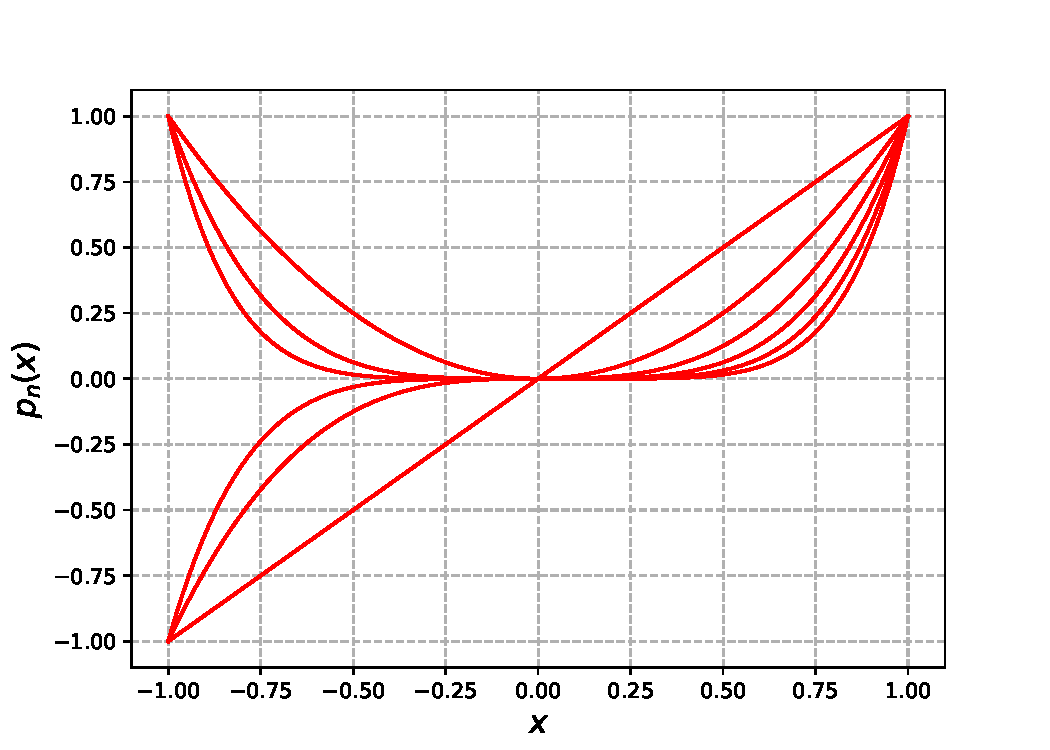
\includegraphics[scale = 0.57]{Figuras/SucesionPolinomios.pdf}
    \caption{Sucesión de polinomios $p_n(x) = x^n, x \in [-1,1]$ para $n = 1, \dots, 6$.}
\end{figure}

Ésta converge en media a $f \equiv 0$. En efecto, 
\begin{align*}
\lim_{n \to + \infty} \int_{-1}^1 |x^n - 0|^2 dx  = \lim_{n \to + \infty }  \int_{-1}^1 x^{2n} \,dx &= \lim_{n \to + \infty} \left. \frac{x^{2n+1}}{2n+1} \right|_{-1}^1 \\
&=  \lim_{n \to + \infty} \frac{2}{2n+1} = 0.
\end{align*}

Sin embargo, no converge puntualmente a $f$ sobre $[-1,1]$, pues 
$$\lim_{n \to + \infty} x^n = \left\{ \begin{array}{cl}
   0 ,& \mbox{si}~ -1 < x < 1 \\
   1  ,&  \mbox{si}~ x = 1 \\
   \mbox{diverge},&  \mbox{si}~ x = -1
\end{array}  \right. .$$

Luego, tampoco uniformemente a $f \equiv 0$ sobre $[-1,1]$.
\end{ejemplo}

\begin{defi}
Considere $f, f_n \in \mathcal{C}[a,b], n \in \mathbb{N}$ y $F_n = \sum\limits_{k=1}^n f_k$. Diremos que la serie $\sum\limits_{n=1}^{\infty} f_n$ \textbf{converge en media} a $f$ si la sucesión de sumas parciales $\{F_n\}_{n\in \mathbb{N}}$ converge en media a $f$. 
\\

\textbf{Notación:} 
$$\sum_{n=1}^{\infty} f_n(t) \sim f(t), \quad t \in [a,b]$$

o 
$$\sum_{n=1}^{\infty} f_n(t) = f(t) ~ [en ~media], \quad t \in [a,b].$$
\end{defi}

\textbf{Observación:}  
\begin{shaded}
$$\sum_{n=1}^{\infty} f_n(t) \sim f(t), \quad t \in [a,b] ~\Leftrightarrow~ \lim_{n \to + \infty} \int_a^b \left[ \sum_{k=1}^n f_k(t) - f(t)\right]^2 \, dt = 0.$$ 
\end{shaded}

\begin{defi}
Una sucesión $\{f_n\}_{n \in \mathbb{N}}$ en $\mathcal{C}[a,b]$ se dice \textbf{sucesión de Cauchy} si dado $\varepsilon > 0$, existe un $N \in \mathbb{N}$ tal que 
$$\forall n,m \geq N ~\Rightarrow~ \norm{f_n-f_m} < \varepsilon.$$
\end{defi}

La definición anterior se puede generalizar a espacios de funciones sin norma, pero con una métrica definida.

Es inmediato verificar que $\{f_n\}_{n \in \mathbb{N}}$ converge a una función $f$ en media, entonces es de Cauchy, pues 
$$\norm{f_n - f_m} \leq \norm{f_n - f} + \norm{f_m - f},$$

y ambos términos en el lado derecho se pueden acotar por un $\varepsilon > 0$ arbitrario para todo $n,m \geq N$. El inverso, sin embargo, es falso, como se puede apreciar en el siguiente ejemplo:

\begin{ejemplo}
Consideremos el conjunto de funciones reales 
 $\mathcal{C}_0[0,1]$, con el producto escalar definido como 
$$\langle f,g\rangle = \int_0^1 f(x) g(x) \,dx.$$

Sea  
\begin{equation*}
    f_n(x) = \left\{ \begin{array}{cl}
       1,  & \mbox{si} ~ 0 \leq x \leq \frac{1}{2}\\
    1 - \left(x - \frac{1}{2} \right)n,     & \mbox{si}  ~ \frac{1}{2} < x < \frac{1}{2} + \frac{1}{n} \\
    0, & \mbox{si} ~ \frac{1}{2} + \frac{1}{n} \leq x \leq 1
    \end{array} \right., n \geq 2.
\end{equation*}

\begin{figure}[H]
    \centering
    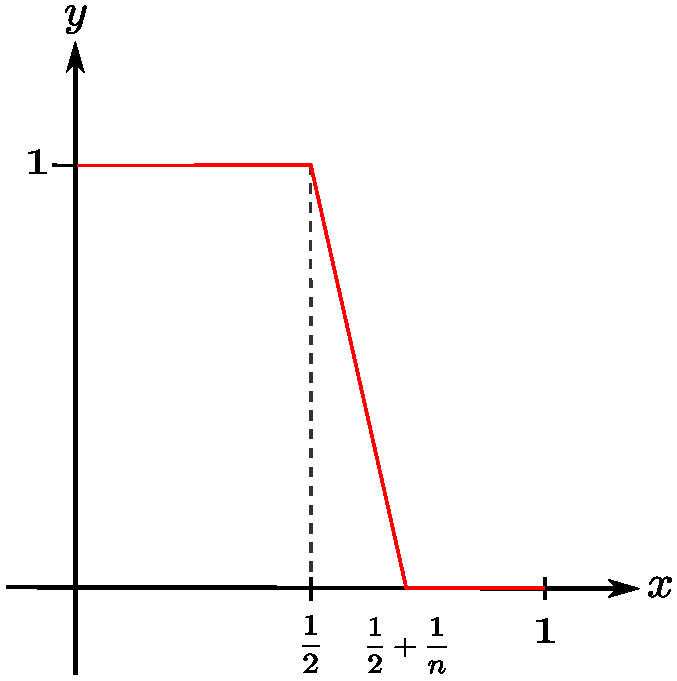
\includegraphics[scale = 0.5]{Figuras/EjemploCauchy.pdf}
    \caption{Ejemplo de sucesión de Cauchy que no converge en media a $C_0[0,1]$.}
\end{figure}

Para $m \geq n$, 
\begin{align*}
    \norm{f_n - f_m}^2 = \int_0^1 |f_n(x) - f_m(x)|^2 \,dx &= \int_0^{\frac{1}{2}} [1-1] \,dx + \int_{\frac{1}{2}}^{\frac{1}{2} + \frac{1}{n}} |f_n(x) - f_m(x)|^2 \,dx + \int_{\frac{1}{2} + \frac{1}{n}}^1 0 \, dx \\
    &=  \int_{\frac{1}{2}}^{\frac{1}{2} + \frac{1}{n}} |f_n(x) - f_m(x)|^2 \,dx.
\end{align*}

Ahora, para todo $x \in \left[\frac{1}{2}, \frac{1}{2}  + \frac{1}{n} \right]$, tenemos

$$|f_n(x) - f_m(x)| \leq |f_n(x)| + |f_m(x)| \leq 1 + 1 = 2. $$

Luego, 
\begin{equation*}
   \norm{f_n - f_m}^2  = \int_{\frac{1}{2}}^{\frac{1}{2} + \frac{1}{n}} |f_n(x) - f_m(x)|^2 \,dx \leq \int_{\frac{1}{2}}^{\frac{1}{2} + \frac{1}{n}} 4 \,dx = \frac{4}{n} ~\Rightarrow~ \norm{f_n - f_m} \leq \frac{2}{\sqrt{n}}.
\end{equation*}

Para $m < n$, es fácil de ver que 
$$\norm{f_n - f_m} \leq \frac{2}{\sqrt{m}}.$$

Así, dado $\varepsilon > 0$, por propiedad arquimediana, existe $N \in \mathbb{N}$ tal que 
$$N > \frac{4}{\varepsilon^2} $$

que verifica 
$$\forall m,n \geq N ~\Rightarrow~   \norm{f_n - f_m} < \varepsilon$$

de modo que es una sucesión de Cauchy. Sin embargo, $\{f_n\}$ converge en media a una función discontinua en $x = \frac{1}{2}$ (pruébelo!), y por lo tanto no converge en $\mathcal{C}_0[0,1]$.
\end{ejemplo}

\begin{defi}
Un espacio normado es llamado \textbf{completo} si toda sucesión de Cauchy es convergente. A un espacio normado completo se le llama \textbf{espacio de Banach}. A un espacio pre-Hilbert que es completo se le llama \textbf{espacio de Hilbert}
\end{defi}

\begin{defi}
El conjunto de funciones $\{\varphi_n(t)\}_{n=0, \pm 1, \pm 2, \dots}$ se dice \textbf{ortogonal} si 
$$\langle \varphi_n , \varphi_m \rangle = 0, \quad \mbox{para} ~ n \neq m.$$

Si además, $\norm{\varphi_n} = 1$ para cada $n \in \mathbb{Z}$, se dice que es un conjunto \textbf{ortonormal}, entonces podemos escribir 
$$\langle \varphi_n , \varphi_m \rangle = \delta_{nm}, \quad \forall n,m.$$
\end{defi}

\begin{ejemplo}
Como ejemplo de funciones ortonormales tenemos las $c_n(t) \in \mathcal{C}_0[-\pi,\pi]$ con $n = 0, \pm 1, \pm 2, \dots$ que se definen como
$$c_n(t) = \frac{1}{\sqrt{2\pi}} e^{i nt}.$$

En efecto, para $n \neq m$, se tiene que
\begin{align*}
    \langle c_n , c_m \rangle = \frac{1}{2\pi} \int_{-\pi}^{\pi} e^{i(n-m)t} \,dt &= \frac{1}{2\pi} \left[ -\frac{i}{n-m} e^{i(n-m) t}\right]_{-\pi}^{\pi} \\
    &= \frac{i}{2\pi(m-n)} [e^{i n\pi} + e^{-i m \pi} - e^{-in \pi} - e^{im \pi}] \\
    &= 0.
\end{align*}

Por otro lado, para $n = m$:
\begin{equation*}
  \langle c_n , c_n \rangle =\frac{1}{2\pi} \int_{-\pi}^{\pi} e^{i(n-n)t} \,dt = \frac{1}{2\pi} \int_{-\pi}^{\pi} 1 \,dt = 1.
\end{equation*}
$$\therefore  \langle c_n , c_m \rangle = \delta_{nm}.$$
\end{ejemplo}

\begin{ejemplo}
Pruebe que el conjunto de funciones 
$$\left\{ \frac{1}{\sqrt{2 \pi}}, \frac{\cos(nt)}{\sqrt{\pi}} ,  \frac{\sin(nt)}{\sqrt{\pi}} \right\}_{n=1}^{\infty}$$

es ortonormal en $\mathcal{C}[-\pi,\pi]$.
\\

\textbf{Solución}: Probemos primero la normalización.
\begin{align*}
    \int_{-\pi}^{\pi} \left( \frac{1}{\sqrt{2\pi}} \right)^2 \,dt &= 1, \\
    \int_{-\pi}^{\pi} \frac{\cos^2(nt)}{\pi} \,dt &=  \frac{1}{\pi} \int_{-\pi}^{\pi} \frac{1}{2} + \frac{1}{2} \cos(2n t) \,dt = 1, \\
    \int_{-\pi}^{\pi} \frac{\sin^2(nt)}{\pi} \,dt &=  \frac{1}{\pi} \int_{-\pi}^{\pi} \frac{1}{2} - \frac{1}{2} \cos(2n t) \,dt = 1.
\end{align*}

Para la ortogonalidad, tengamos en cuenta las siguientes identidades trigonométricas:
\begin{align*}
    \sin \alpha \sin \beta &= \frac{1}{2} [\cos(\alpha - \beta) - \cos(\alpha + \beta)], \\
    \cos \alpha \cos \beta &= \frac{1}{2} [\cos(\alpha - \beta) + \cos(\alpha + \beta)], \\
    \sin \alpha \cos \beta &= \frac{1}{2} [\sin(\alpha + \beta) + \sin(\alpha - \beta)].
\end{align*}

Entonces, 
\begin{align*}
    \int_{-\pi}^{\pi} \frac{1}{\sqrt{2} \pi} \cos(nt) \,dt &=  \left. \frac{1}{\sqrt{2}\pi n} \sin(nt) \right|_{-\pi}^{\pi} = 0, \\
     \int_{-\pi}^{\pi} \frac{1}{\sqrt{2} \pi} \sin(nt) \,dt &=   \left. - \frac{1}{\sqrt{2}\pi n} \cos(nt) \right|_{-\pi}^{\pi} = 0,\\
      \int_{-\pi}^{\pi} \frac{1}{\pi} \cos(n t) \sin(m t)\,dt &=  \frac{1}{2 \pi} \int_{-\pi}^{\pi} \sin(m+n)t + \sin(m-n)t \ dt = 0; \quad n,m \in \mathbb{N}. 
\end{align*}

Para todo $n, m \in \mathbb{N}$, $m \neq n$, se tiene que 
\begin{align*}
    \int_{-\pi}^{\pi} \frac{1}{\pi} \cos(n t) \cos(mt) \,dt &= \frac{1}{2\pi} \int_{-\pi}^{\pi} \cos(n-m)t + \cos(n+m) t\,dt \\
    &= \frac{1}{2\pi} \left[ \frac{1}{n-m} \sin(n-m)t + \frac{1}{n+m} \sin(n+m)t \right]_{-\pi}^{\pi} = 0. \\
     \int_{-\pi}^{\pi} \frac{1}{\pi} \sin(n t) \sin(mt) \,dt &=\frac{1}{2\pi} \int_{-\pi}^{\pi} \cos(n-m)t - \cos(n+m) t\,dt  \\
    &= \frac{1}{2\pi} \left[ \frac{1}{n-m} \sin(n-m)t - \frac{1}{n+m} \sin(n+m)t \right]_{-\pi}^{\pi} = 0.
\end{align*}

Por lo tanto, 
$$\left\{ \frac{1}{\sqrt{2 \pi}}, \frac{\cos(nt)}{\sqrt{\pi}} ,  \frac{\sin(nt)}{\sqrt{\pi}} \right\}_{n=1}^{\infty}$$

es ortonormal en $\mathcal{C}[-\pi,\pi]$.
\end{ejemplo}

\begin{defi}
Sea $S = \{\varphi_n(t)\}_{n=0, \pm 1, \pm 2, \dots}$. Se dice que $S$ es \textbf{linealmente independiente} (l.i.) si todo subconjunto finito de $S$ también lo es.
\end{defi}

\begin{propo} \label{LIortogonal}
Todo conjunto ortogonal en $\mathcal{C}[a,b]$ que no contenga al vector nulo es linealmente independiente.
\end{propo}

\begin{demo}
Sea $S = \{\varphi_n(t)\}_{n=0, \pm 1, \pm 2, \dots}$ ortogonal tal que $\varphi_n \not\equiv 0, \forall n$. Consideremos el subconjunto finito de $S$, $S' = \{\varphi_{i_1}, \dots, \varphi_{i_n}\}$ y además la combinación lineal
$$\alpha_1 \varphi_{i_1} + \alpha_2 \varphi_{i_2} + \cdots + \alpha_n \varphi_{i_n} \equiv 0.$$

Entonces, para un cierto $\varphi_{i_m}$, se tiene que
$$\langle \alpha_1 \varphi_{i_1} + \alpha_2 \varphi_{i_2} + \cdots + \alpha_n \varphi_{i_n},\varphi_{i_m} \rangle = \alpha_m \underbrace{\norm{\varphi_{i_m}}^2}_{\neq 0} = 0.$$

Por lo tanto, 
$$\alpha_m = 0, \quad m = 1, 2, \dots, n$$

probando así que $S'$ es linealmente independiente y en consecuencia $S$ es l.i.
\end{demo}

\section{Proceso de ortonormalización de Gram-Schmidt}

Sea $\{v_n\}_{n = 1,2, \dots}$ un conjunto linealmente independiente de funciones en $\mathcal{C}[a,b]$. Para construir un conjunto ortonormal debemos seguir los siguientes pasos:

\begin{enumerate}
    \item Construimos 
    $$\varphi_1 = \frac{v_1}{\norm{v_1}}$$ 
    
    tal que $\langle \varphi_1 , \varphi_1 \rangle = 1$. 
    
    \item Consideramos
    $$\overline{\varphi}_2 = v_2 - \langle v_2, \varphi_1   \rangle \varphi_1.$$
    
    Entonces, 
    $$\langle \overline{\varphi}_2, \varphi_1 \rangle = \langle v_2, \varphi_1 \rangle - \langle  v_2, \varphi_1  \rangle \langle \varphi_1, \varphi_1 \rangle = \langle v_2, \varphi_1 \rangle -  \langle  v_2, \varphi_1 \rangle  = 0.$$
    
    Normalizando, 
    $$\varphi_2 = \frac{\overline{\varphi}_2}{\norm{\overline{\varphi}_2}}.$$
    
    \item En general para un cierto $n \geq 2$, consideremos 
 $$\overline{\varphi}_n = v_n - \sum_{j=1}^{n-1} \langle  v_n, \varphi_j \rangle \varphi_j.$$
    
Entonces, para $1 \leq  i \leq n-1$, tenemos que
\begin{align*}
    \langle \Bar{\varphi}_n , \varphi_i \rangle &= \langle v_n , \varphi_i \rangle - \sum_{j=1}^{n-1} \langle v_n , \varphi_j \rangle \langle \varphi_j , \varphi_i\rangle \\
    &= \langle v_n, \varphi_i \rangle - \sum_{j=1}^{n-1} \langle v_n , \varphi_j \rangle \delta_{ji} \\
    &= \langle v_n , \varphi_i \rangle -  \langle v_n, \varphi_i \rangle = 0.
\end{align*}
    
Finalmente, normalizando    
$$\varphi_n = \frac{\overline{\varphi}_n}{\norm{\overline{\varphi}_n}}.$$
\end{enumerate}

El conjunto de funciones $\{\varphi_n\}_{n = 1,2, \dots}$ construido de la manera anterior es un conjunto ortonormal.

Geométricamente, el método se encuentra ilustrado en la figura \ref{fig:Gram-Schmidt}, donde se ha considerado las funciones como vectores y solo el proceso de ortogonalización.

\begin{figure}[H]
    \centering
    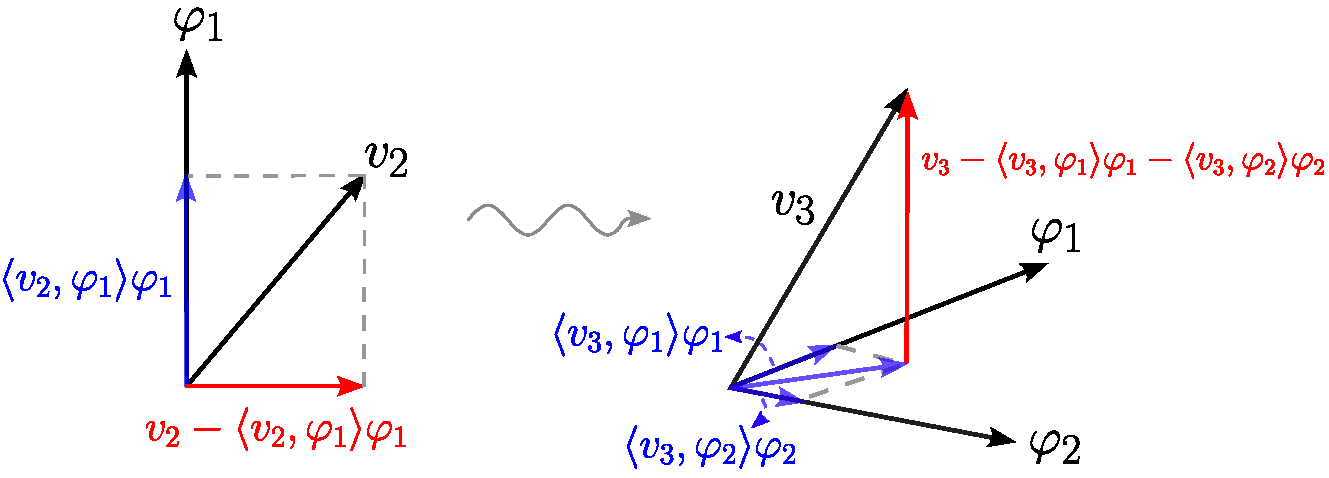
\includegraphics[scale = 0.7]{Figuras/Gram-Schmidt.pdf}
    \caption{Proceso de ortogonalización (sin la normalización) de Gram-Schmidt para tres funciones $\{v_1,v_2,v_3\}$.}
    \label{fig:Gram-Schmidt}
\end{figure}

\newpage
\section{Coeficientes de Fourier}

Ahora, definiremos un espacio de funciones más general que $\mathcal{C}[a,b]$, las funciones cuadrado integrables. \footnote{La condición de cuadrado integrable es usada, por ejemplo, en Mecánica Cuántica, pues constituye la base para que las funciones de onda describan el comportamiento de los sistemas físicos, consecuencia de la interpretación de Copenhague (probabilística) de la mecánica cuántica.}

\begin{defi}
    Definimos $\mathcal{L}^2[a,b]$ como el espacio de funciones $f:[a,b] \rightarrow \mathbb{C}$, tales que 
    $$\int_a^b |f(t)|^2 \,dt < \infty.$$
\end{defi}

\begin{teorema}
El espacio $\mathcal{L}^2[a,b]$ es un espacio vectorial con producto interno 
$$\langle f,g \rangle = \int_a^b f(t) g^* (t) \,dt$$

y norma
$$\norm{f} = \left( \int_a^b |f(t)|^2 \,dt \right)^{1/2}.$$
\end{teorema}

La demostración requiere verificar las propiedades del producto interno (escalar) dadas por \ref{ProductoEscalar}, la cual está fuera de los alcances de los contenidos de este apunte. \footnote{Para más información puede consultar bibliografía relacionada a la integral de Lebesgue.} 

\textbf{Observación:} Las funciones seccionalmente continuas son funciones cuadrado integrables.
\\

Sea $\{\varphi_{\nu}(t)\}_{\nu \in \mathbb{N}}$ un conjunto ortonormal de funciones tales que $\varphi_{\nu} \in \mathcal{C}[a,b]$ para todo $\nu \in \mathbb{N}$. Sea $f(t)$ una función cuadrado integrable en $[a,b]$. Deseamos aproximar $f(t)$ por una suma finita 
$$S_n(t) = \sum_{\nu = 1}^n C_{\nu} \varphi_{\nu}(t),$$

de manera que $\norm{f - S_n}$ sea mínimo. Es decir, el objetivo es encontrar los coeficientes $C_{\nu}$ de modo que el \textbf{error cuadrático medio}
$$M_n(f) = \norm{f-S_n}^2 = \int_a^b \left| f(t) - \sum_{\nu = 1}^n C_{\nu} \varphi_{\nu}(t) \right|^2 \,dt,$$

sea mínimo. Evaluemos el error cuadrático medio
\begin{align}
    M_n(f) &= \int_a^b \left( f(t) - \sum_{\nu = 1}^n C_{\nu} \varphi_{\nu}(t)  \right) \left( f(t) - \sum_{\nu = 1}^n C_{\nu} \varphi_{\nu}(t) \right)^* \,dt \nonumber \\
    &= \int_a^b |f(t)|^2 \, dt  + \sum_{\nu = 1}^n |C_{\nu}|^2 \int_a^b |\varphi_{\nu}(t)|^2 \,dt - \sum_{\nu = 1}^n C_{\nu}^* \int_a^b f(t) \varphi_{\nu}^*(t) \,dt \nonumber \\
    & \quad - \sum_{\nu = 1}^n C_{\nu} \int_a^b f^*(t) \varphi_{\nu}(t) \,dt  \nonumber \\
    &= \norm{f}^2 + \sum_{\nu = 1}^n |C_{\nu}|^2 - \sum_{\nu = 1}^n C_{\nu}^* \langle f, \varphi_{\nu} \rangle - \sum_{\nu = 1}^n C_{\nu} \langle f, \varphi_{\nu} \rangle^* + \sum_{\nu = 1}^n |\langle f, \varphi_{\nu} \rangle|^2 - \sum_{\nu = 1}^n |\langle f, \varphi_{\nu} \rangle|^2\nonumber  \\
    &= \norm{f}^2  - \sum_{\nu = 1}^n |\langle f, \varphi_{\nu} \rangle|^2 + \sum_{\nu = 1}^n |C_{\nu} - \langle f , \varphi_{\nu} \rangle|^2 \geq 0, \label{ErrorMedio}
\end{align}

ya que la norma es mayor o igual a cero siempre. Claramente el mínimo se obtiene cuando $C_{\nu} = \langle f, \varphi_{\nu} \rangle$. 

De lo anterior se desprende: 
\begin{shaded}
 \begin{equation}
 \sum_{\nu = 1}^n |C_{\nu}|^2 = \sum_{\nu = 1}^n |\langle f , \varphi_{\nu} \rangle|^2 \leq \norm{f}^2  \qquad \mbox{\textbf{Desigualdad de Bessel}} \label{D.Bessel}.
\end{equation}
 
\end{shaded}

Como el número a la derecha de la desigualdad es independiente de $n$, la suma está acotada superiormente. Siendo todos sus términos no negativos, tenemos que
$$\sum_{\nu = 1}^{\infty} |C_{\nu}|^2 < \infty ~\Rightarrow~ \lim_{\nu \to + \infty} |C_{\nu}|^2 = 0 ~\Rightarrow ~ \lim_{\nu \to + \infty} \langle f , \varphi_{\nu} \rangle = 0.$$

Luego,
\begin{equation*}
 \sum_{\nu = 1}^{\infty} |C_{\nu}|^2 = \sum_{\nu = 1}^{\infty} |\langle f , \varphi_{\nu} \rangle|^2 \leq \norm{f}^2    .
\end{equation*}

\begin{defi}
Los coeficientes $\langle f , \varphi_{\nu}\rangle$ son llamados los \textbf{coeficientes de Fourier} de $f$  respecto al sistema ortonormal $\{\varphi_{\nu}\}_{\nu = 1,2, \dots}$. La serie $\sum\limits_{\nu = 1}^{\infty} C_{\nu} \varphi_{\nu}(t)$ se llama \textbf{serie generalizada de Fourier} de $f$ relativa al sistema ortonormal $\{\varphi_{\nu}\}_{\nu = 1,2, \dots}$.

\end{defi}

\begin{defi}
Si un conjunto de funciones $\{\varphi_{\nu}\}$ en cierto espacio permite aproximar en la norma (en media), con sus combinaciones lineales, cualquier función $f$ del espacio tan bien como se quiera, es decir,
$$\left\Vert f - \sum_{\nu} C_{\nu} \varphi_{\nu} \right\Vert< \varepsilon, \qquad \mbox{para $\varepsilon$ arbitrario},$$

se dice que es un \textbf{conjunto completo} respecto a este espacio.
\end{defi}

Sean $C_{\nu} = \langle f , \varphi_{\nu} \rangle$ los coeficientes de Fourier de $f$ respecto del conjunto ortonormal  $\{\varphi_{\nu}\}$, entonces la completitud de este conjunto se puede expresar por 
$$\lim_{n \to + \infty} \left\Vert f - \sum_{\nu =1}^{n} C_{\nu} \varphi_{\nu} \right\Vert = 0,$$

es decir, 
$$f \sim \sum_{\nu = 1}^{\infty} C_{\nu} \varphi_{\nu}.$$

Lo anterior NO implica que $f(t) = \sum\limits_{\nu = 1}^{\infty} C_{\nu} \varphi_{\nu}(t)$ en algún otro sentido (convergencia puntual o uniforme). Si
$$f \sim \sum_{\nu = 1}^{\infty} C_{\nu} \varphi_{\nu},$$

entonces de la relación \eqref{ErrorMedio}, tenemos 
\begin{equation*}
    \lim_{n \to + \infty} \left\Vert f - \sum_{\nu = 1}^n  C_{\nu} \varphi_{\nu} \right\Vert^2 = \lim_{n \to + \infty} \left\{ \Vert f \Vert^2 - \sum_{\nu = 1}^{n} |C_n|^2 \right\} = \norm{f}^2  - \sum_{\nu = 1}^{\infty} |C_n|^2 = 0.
\end{equation*}

Lo que implica que
\begin{shaded}
 \begin{equation}
    \norm{f}^2  = \sum_{\nu =1 }^{\infty} |C_{\nu}|^2 \qquad \mbox{\textbf{Igualdad de Parseval}}
\end{equation}   
\end{shaded}

\textbf{Observación:} El conjunto ortogonal completo $\{\varphi_{\nu}\}$ se le conoce también como \textbf{base ortogonal} del espacio de funciones en cuestión.

\begin{ejemplo}
El conjunto $\left\{ \frac{1}{\sqrt{2 \pi}} e^{i n t} \right\}_{n \in \mathbb{Z}}$ es ortonormal completo respecto a $[-\pi,\pi]$.
$$f(t) \sim \sum_{n = - \infty}^{\infty} C_n \frac{e^{int}}{\sqrt{2\pi}} ~\Rightarrow~ \int_{-\pi}^{\pi} |f|^2 \,dt = \sum_{n=- \infty}^{\infty} |C_n|^2 = \norm{f}^2 .$$
\end{ejemplo}


\begin{teorema}{}{} 
Si el conjunto ortonormal $\{\phi_{\nu}\}$ es completo respecto a $\mathcal{C}[a,b]$, entonces en $\mathcal{C}[a,b]$ la única función ortonormal a todo $\varphi_{\nu}$ es $f(t) \equiv 0$.
\end{teorema}

\begin{demo}
Sea $f$ una función ortonormal a todo $\varphi_{\nu}$, si $f(t_0) \neq 0$ para algún $t_0 \in [a,b]$, la función también es no nula en una vecindad en torno a $t_0$ (por continuidad), por lo tanto 
$$\int_a^b |f(t)|^2 \,dt = \norm{f}^2  > 0,$$

pero usando la igualdad de Parseval, tenemos para la norma de $f$ que
$$\norm{f}^2  = \sum_{\nu} |C_{\nu}|^2 = \sum_{\nu} |\langle f ,\varphi_{\nu} \rangle|^2 > 0,$$

es decir, $f$ no es ortogonal a todos los $\varphi_{\nu}$, lo cual es una contradicción. Luego, $f$ debe ser idénticamente nula.
\end{demo}

\begin{teorema}
Sea $\{S_n(t) \in \mathcal{C}_0[a,b]\}$; si existe $F(t)$ tal que la sucesión $S_n(t) = \sum\limits_{\nu = 1}^n C_{\nu} \varphi_{\nu}(t)$ converge uniformemente a $F(t)$, entonces $F(t)$ es continua, es decir, $F(t) \in \mathcal{C}_0[a,b]$.
\end{teorema}

\begin{demo}
Por convergencia uniforme, dado $\varepsilon > 0$, $\exists N \in \mathbb{N}$ tal que
$$n \geq N \wedge \forall t \in [a,b] ~\Rightarrow~ |S_n(t) - F(t)| < \frac{\varepsilon}{3}.$$

Además, por la continuidad de $S_n$ para todo $t_0 \in [a,b]$, existe $\delta(\varepsilon, N, t_0)$ tal que
$$\forall t \in [a,b]: ~ 0 < |t-t_0| < \delta ~\Rightarrow~ |S_N(t) - S_N(t_0)| < \frac{\varepsilon}{3}.$$

Por lo tanto, 
\begin{align*}
 \forall t \in [a,b]: ~ 0 < |t-t_0| < \delta &\Rightarrow |F(t) - F(t_0)|  \\
 &= |F(t) - S_n(t) + S_n(t) - S_n(t_0) + S_n(t_0) - f(t_0)| \\
 &\leq |F(t) - S_n(t)| + |S_n(t) - S_n(t_0)| + |S_n(t_0) - F(t_0)| \\
 &\leq \frac{\varepsilon}{3} + \frac{\varepsilon}{3} + \frac{\varepsilon}{3} = \varepsilon .
\end{align*}
\end{demo}

Este teorema nos asegura que una función discontinua no puede ser aproximada uniformemente por una familia de funciones continuas (por ejemplo, las funciones sinusoidales).

\begin{teorema}
Si dos funciones $f,g \in \mathcal{C}[a,b]$ tienen igual expansión en base completa (en el sentido de aproximación en la norma), entonces $f(t) = g(t)$.
\end{teorema}

\begin{demo}
Sea
$$S(t) = \sum_{\nu = 1}^{\infty} \langle f, \varphi_{\nu}\rangle \varphi_{\nu}(t)$$

la aproximación en la norma para $f$ y $g$. Luego, 
$$\Vert f-S \Vert = \Vert g-S \Vert = 0.$$

Así, 
\begin{equation*}
    \Vert f-g \Vert = \Vert f-S+S-g \Vert \leq \Vert f-S \Vert + \Vert S-g \Vert = 0 +0 = 0 ~\Rightarrow~ f = g.
\end{equation*}

\end{demo}

\section{Convergencia según Cesàro*}

Si consideramos la serie
$$\frac{1}{1-x} = \sum_{n=1}^{\infty} x^{n-1} = 1 + x + x^2 + x^3 + \cdots$$

ella converge para $|x|< 1$. A pesar de lo anterior evaluemos la función y su expansión en serie en $x = -1$:
$$\left. \frac{1}{1-x} \right|_{x= -1} \overset{?}{=} \frac{1}{2} = 1 - 1 + 1 -1 +1 -1 + \cdots$$

¿Será posible sumar la serie de modo que ésta sí converja al valor de la función en ese punto?

\begin{defi}
Sea $s_n$ la suma parcial $n$-ésima de la serie $\sum\limits_{n=1}^{\infty} a_n$ y sea $\{\sigma_n\}_{n\in \mathbb{N}}$ la sucesión de las medias aritméticas definidas por
$$\sigma_n = \frac{s_1 + \cdots + s_n}{n}, \quad n = 1, 2, \dots$$

La serie $\sum\limits_{n=1}^{\infty} a_n$ es \textbf{sumable de Cesàro} si $\{\sigma_n\}_{n\in \mathbb{N}}$ converge. Si $\lim\limits_{n \to + \infty} \sigma_n = S^*$, entonces $S^*$ se llama \textbf{suma de Cesàro} de $\sum\limits_{n=1}^{\infty} a_n$ y se escribe 
$$ \sum_{n=1}^{\infty} ^*   a_n = S^*.$$
\end{defi}

\begin{ejemplo}
Sea $a_n = x^{n-1}$ con $x \neq 1$. Entonces
$$s_n = \frac{1}{1-x} - \frac{x^n}{1-x} \qquad \mbox{(Demuéstrelo!!)}$$

y
\begin{align*}
 \sigma_n = \frac{1}{n} \sum_{k=1}^n \left\{\frac{1}{1-x} - \frac{x^k}{1-x} \right\} &= \frac{1}{1-x} - \frac{1}{n(1-x)} \sum_{k =1}^{n} x^k   \\
 &=\frac{1}{1-x} -  \frac{1}{n} \frac{x(1-x^n)}{(1-x)^2}.
\end{align*}

Por consiguiente, 
$$\sum_{n=1}^{\infty}^* x^{n-1} = \lim_{n \to +\infty} \left\{ \frac{1}{1-x} -  \frac{1}{n} \frac{x(1-x^n)}{(1-x)^2}\right\} = \frac{1}{1-x}; \quad |x| \leq 1, x \neq 1. $$

En particular,
$$\sum_{n=1}^{\infty}^* (-1)^{n-1} = \frac{1}{2}.$$

\end{ejemplo}

Note que la idea de la definición de sumabilidad de Cesàro es encontrar una forma de dar significado a series que en otro caso serían divergentes.
\\

\textbf{Observación}: La convergencia ordinaria necesita que el $\lim\limits_{n \to + \infty} \sum\limits_{k = 1}^n a_{k}$ exista. 

\hspace{2.45cm} La convergencia según Cesàro necesita que el $\lim\limits_{n \to + \infty} \frac{1}{n} \sum\limits_{k = 1}^n  \sum\limits_{l = 1}^{k} a_{l}$ exista.

\begin{teorema}
Si una serie es convergente con suma $S$, entonces es sumable de Cesàro con suma $S^* = S$.
\end{teorema}

Problemas similares a la serie discreta anterior ofrece calcular la integral, desde cero hasta infinito, de una función oscilante, que no decrece, del tipo $\int_0^{\infty} \sin(\omega x) \,dx$.

En el espíritu del caso discreto, proponemos la siguiente definición.

\begin{defi}
Definimos una \textbf{integral de Cesàro} de la siguiente manera:
\begin{equation}
    ^* \int_0^{\infty} f(t) \,dt = \lim_{y \to \infty } \frac{1}{y} \left\{ \int_0^y \int_0^x f(t) \,dt dx \right\}. \label{IntegralCesaro1}
\end{equation}

\end{defi}


Podemos encontrar una expresión alternativa para la integral de Cesàro integrando por partes la ecuación \eqref{IntegralCesaro1}:
\begin{align*}
    ^* \int_0^{\infty} f(t) \,dt &= \lim_{y \to \infty } \frac{1}{y} \left\{ \int_0^y \int_0^x f(t) \,dt dx \right\} \\
    &= \lim_{y \to \infty } \frac{1}{y} \left\{\left. x \int_0^x f(t)\,dt \right|_0^y - \int_0^y x f(x) \,dx \right\} \\
    &= \lim_{y \to \infty } \frac{1}{y} \left\{ y \int_0^y f(t) \,dt - \int_0^y xf(x) \,dx \right\}
\end{align*}
\begin{equation}
    \Rightarrow ~  \boxed{^* \int_0^{\infty} f(t) \,dt = \lim_{y \to \infty} \int_0^y \left( 1 - \frac{x}{y} \right) f(x) \,dx} \label{IntegralCesaro2}
 \end{equation}
 
 \begin{ejemplo}
Evalúe la integral de Cesàro de la función $f(x) = \sin(\omega x)$ con $\omega \neq 0$.
\\

\textbf{Solución:} Usando la ecuación \eqref{IntegralCesaro1}, obtenemos que
\begin{align*}
      ^* \int_0^{\infty} \sin(\omega t) \,dt &= \lim_{y \to \infty } \frac{1}{y} \left\{ \int_0^y \int_0^x \sin(\omega t) \,dt dx \right\} \\
      &= \lim_{y \to \infty } \frac{1}{y} \int_0^y \left[ \frac{1 - \cos(\omega x)}{\omega}\right] \, dx \\
      &= \lim_{y \to \infty} \left[ \frac{1}{\omega} - \frac{1}{\omega^2} \frac{\sin(\omega y)}{y}\right]
\end{align*}
\begin{equation}
    \Rightarrow ~  \boxed{^* \int_0^{\infty} \sin(\omega t) \,dt = \frac{1}{\omega}} \label{CesaroSeno}
 \end{equation}

 \end{ejemplo}
 
  \begin{ejemplo}
Evalúe la integral de Cesàro de la función $f(x) = \cos(\omega x)$ con $\omega \neq 0$.
\\

\textbf{Solución:} Usando la ecuación \eqref{IntegralCesaro1}, obtenemos que
\begin{align*}
      ^* \int_0^{\infty} \cos(\omega t) \,dt &= \lim_{y \to \infty } \frac{1}{y} \left\{ \int_0^y \int_0^x \cos(\omega t) \,dt dx \right\} \\
      &= \lim_{y \to \infty } \frac{1}{y} \int_0^y \frac{\sin(\omega x)}{\omega} \, dx \\
      &= \lim_{y \to \infty} \left[ \frac{1}{\omega^2 y} - \frac{\cos(\omega y)}{\omega^2 y} \right]
\end{align*}
\begin{equation}
    \Rightarrow ~  \boxed{^* \int_0^{\infty} \cos(\omega t) \,dt = 0 } \label{CesaroCoseno}
 \end{equation}

 \end{ejemplo}
\chapter{Análisis de Fourier}

\section{Periodicidad y paridad de funciones}

\subsection{Funciones periódicas}

\begin{defi}
Una función $f: \mathbb{R} \longrightarrow \mathbb{C} $ se dice que es \textbf{periódica de período $T$}, $T\neq 0$, si 
\begin{equation}
f(t) = f(t +T ), \quad \forall t.    \label{Periodica}
\end{equation}

La constante $T$ la tomaremos como la  menor constante positiva que satisface la igualdad \eqref{Periodica}.
\end{defi}

\textbf{Observación:} No es difícil de ver que se verifica:

\begin{enumerate}
    \item $$f(t) = f(t + nT), \quad n = 0, \pm 1, \pm 2, \dots$$
    
    \item Si $f(t)$ y $g(t)$ son funciones periódicas de período $T$, entonces la función
    $$h(t) = \alpha f(t) + \beta g(t); \quad \alpha, \beta \in \mathbb{C},$$
    
    tiene el mismo período $T$.
\end{enumerate}

\begin{ejemplo}
Encontrar el período de la función $f(t) = \cos \frac{t}{3} + \cos \frac{t}{4}$.
\\

\textbf{Solución:} Si la función $f(t)$ es periódica con período $T$, entonces, de \eqref{Periodica},
$$\cos \frac{1}{3}(t + T) + \cos \frac{1}{4}(t + T) = \cos \frac{t}{3} + \cos \frac{t}{4}.$$

Como $\cos(\theta + 2\pi n) = \cos \theta, n \in \mathbb{Z}$, obtenemos que 
$$\frac{1}{3} T = 2\pi n, \quad \frac{1}{4}T = 2\pi m; \quad n,m \in \mathbb{Z}.$$

Por consiguiente $T = 6\pi n = 8\pi m$; cuando $n = 4$ y $m=3$, se obtiene el mínimo valor de $T$. Así, $T = 24\pi$.
\end{ejemplo}

En general, si la función 
$$f(t) = \cos (\omega_1 t) + \cos (\omega_2 t)$$

es periódica de período $T$, entonces es posible encontrar dos enteros $n$ y $m$ tales que 
\begin{align}
    \omega_1 T &= 2\pi n,  \label{Periodica1}\\
     \omega_2 T &= 2\pi m. \label{Periodica2}
\end{align}

El cociente de \eqref{Periodica1} y \eqref{Periodica2} es
$$\frac{\omega_1}{\omega_2} = \frac{n}{m},$$

es decir, la relación $\omega_1/ \omega_2$ debe ser un número racional.

\begin{propo}
Sea $f: \mathbb{R} \longrightarrow \mathbb{C}$ una función periódica de período $T$. Sea $a \in \mathbb{R}$, entonces
$$ \int_{a-T/2}^{a + T/2} f(t) \,dt = \int_{- T/2}^{T/2} f(t) \,dt .$$
\end{propo}

\begin{demo}
Utilizando la propiedad de aditividad de la integral compleja:
\begin{equation*}
    \int_{a-T/2}^{a + T/2} f(t) \,dt = \int_{a - T/2}^{-T/2} f(t) \,dt + \int_{- T/2}^{a + T/2} f(t) \,dt.
\end{equation*}

Haciendo la sustitución  $t = t' - T ~\Rightarrow~ dt = dt'$ en la primera integral, obtenemos
\begin{align*}
   \int_{a - T/2}^{-T/2}f(t) \,dt + \int_{- T/2}^{a + T/2} f(t) \,dt   &= \int_{a + T/2}^{T/2} f(t'-T) \,dt' + \int_{- T/2}^{a + T/2} f(t) \,dt \\
   &= \int_{a + T/2}^{T/2} f(t'-T + T) \,dt' + \int_{- T/2}^{a + T/2} f(t) \,dt \\
   &= \int_{a + T/2}^{T/2} f(t') \,dt' + \int_{-T/2}^{a + T/2} f(t) \,dt \\
   &= \int_{-T/2}^{T/2} f(t) \,dt.
\end{align*}
\end{demo}

\begin{defi}
Sea $f: [a,b] \rightarrow \mathbb{R}$ seccionalmente continua, se llama \textbf{extensión periódica} de $f$ a la función $f_e: \mathbb{R} \rightarrow \mathbb{R}$,
$$f_e(t) = f(t + k_0 (b-a))$$

donde $k_0 \in \mathbb{Z}$ es el único entero que verifica $t + k_0(b-a) \in [a,b].$
\end{defi}

\begin{ejemplo}
La extensión periódica de $f \in \mathcal{C}[-\pi,\pi]$ real es
$$f_e(t) = f_e(t + 2\pi)$$

\begin{figure}[H]
    \centering
    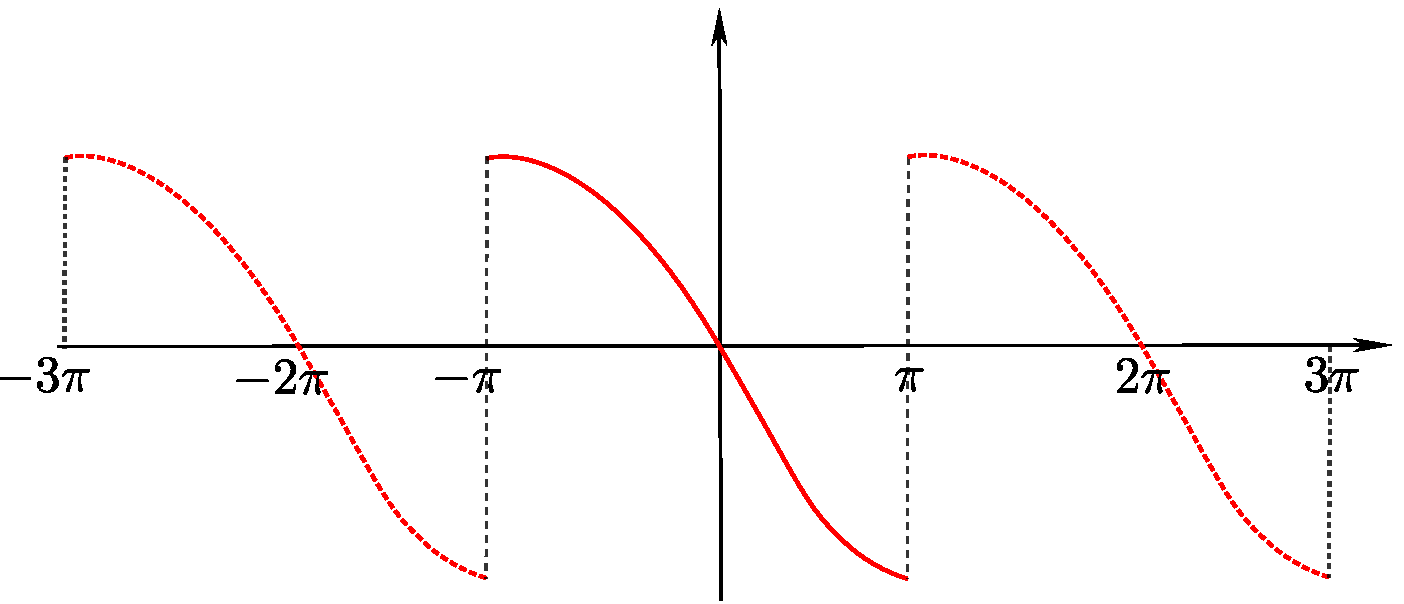
\includegraphics[scale = 0.45]{Figuras/Periocidad.pdf}
    \caption{Extensión periódica de una función real seccionalmente continua en $[-\pi,\pi]$.}
\end{figure}
\end{ejemplo}

\subsection{Funciones pares e impares}
 
\begin{defi}
Sea $f: [-a,a] \longrightarrow \mathbb{R}$ perteneciente a $\mathcal{C}[-a,a]$.
\vspace{-0.1cm}
\begin{align*}
    f ~\mbox{es par} &\Leftrightarrow \forall x \in [-a,a] :~ f(-t) = f(t). \\
    f ~\mbox{es impar} &\Leftrightarrow \forall x \in [-a,a] :~ f(-t) = -f(t).
\end{align*}
\end{defi} 

\textbf{Observación 1:} Sea $f: [-a,a] \longrightarrow \mathbb{R}$ integrable,
\begin{align*}
    f ~\mbox{es par} &\Rightarrow \int_{-a}^a f(t) \,dt = 2 \int_0^a f(t) \,dt. \\
    f ~\mbox{es impar} &\Rightarrow \int_{-a}^a f(t) \,dt = 0.
\end{align*}

\textbf{Observación 2:} Toda función $f:[-a,a] \longrightarrow \mathbb{R}$ puede expresarse como la suma de una función par más otra impar: $f = f_p + f_i$ con 
$$f_p(t) = \frac{f(t) + f(-t)}{2}, \quad f_i(t) = \frac{f(t) - f(-t)}{2}.$$

\begin{defi}
Sea $f \in \mathcal{C}[0,a]$ real, entonces la \textbf{extensión par} y la \textbf{extensión impar} de $f$ están definidas, respectivamente, por:
\begin{equation*}
    E_f(t) = \left\{ \begin{array}{cll}
    f(-t)     & \mbox{si} & -a \leq t < 0 \\
    f(t)     & \mbox{si} & 0 \leq t \leq a
    \end{array} \right. , ~ O_f(t) = \left\{ \begin{array}{cll}
    -f(-t)     & \mbox{si} & -a \leq t < 0 \\
    f(t)     & \mbox{si} & 0 \leq t \leq a
    \end{array} \right. .
\end{equation*}
\end{defi}

\begin{figure}[H]
    \centering
    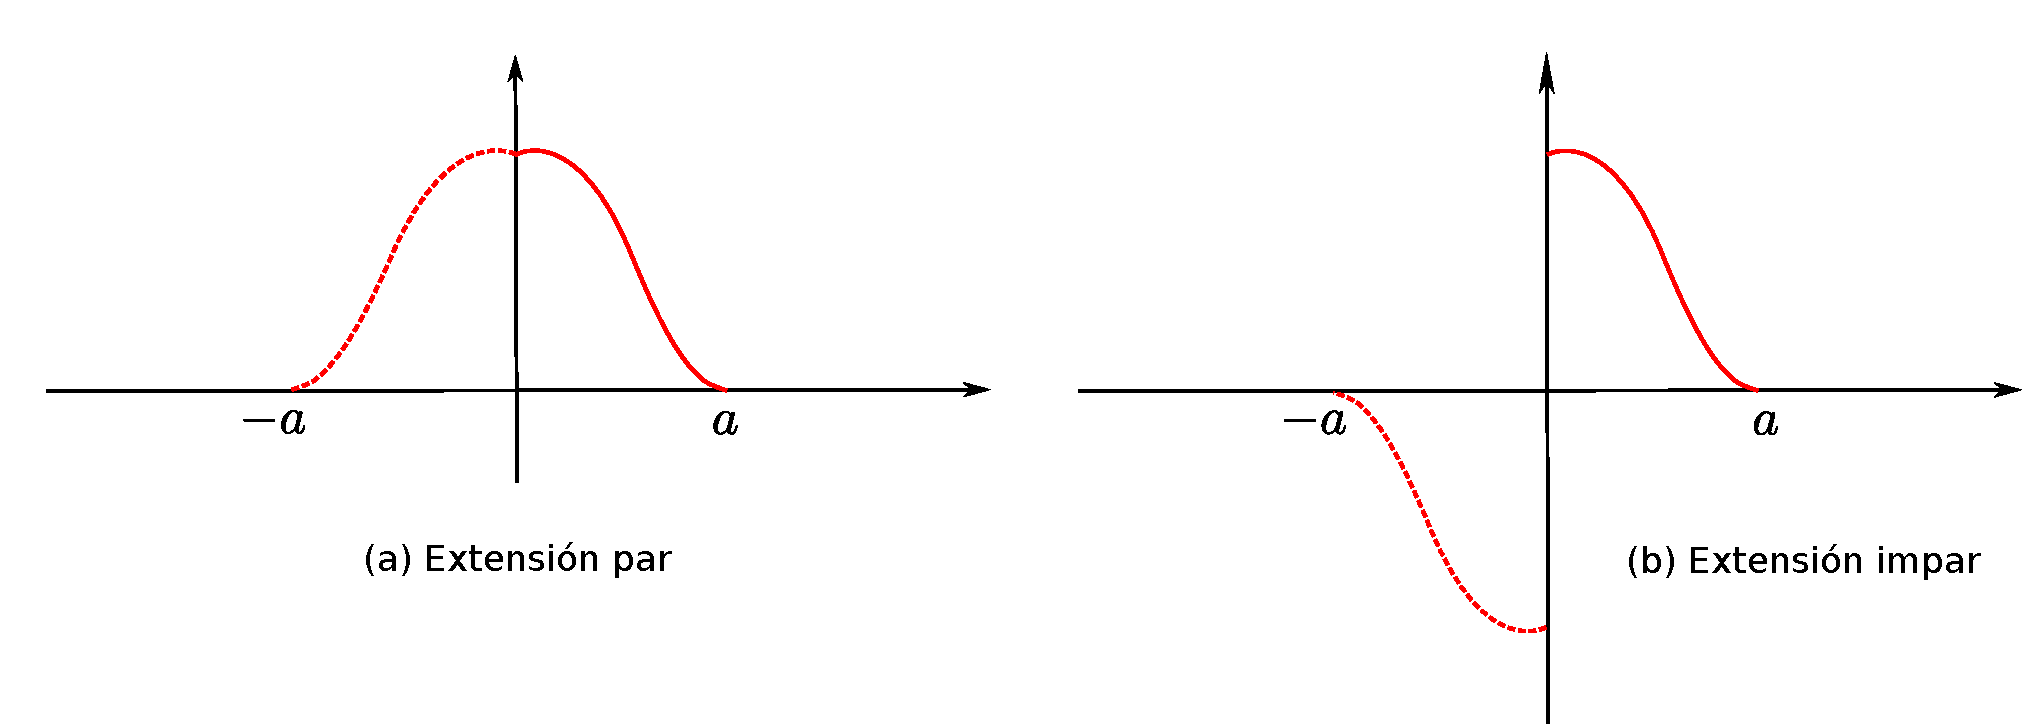
\includegraphics[scale = 0.45]{Figuras/Paridad.pdf}
    \caption{Extensión par e impar de una función real seccionalmente continua en $[0,a]$. }
\end{figure}

\section{Serie de Fourier trigonométrica}

\subsection{Definición}

En el espacio $\mathcal{C}[-\pi,\pi]$ consideremos el sistema ortonormal completo 
$$\left\{ \frac{1}{\sqrt{2\pi}}, \frac{\cos(nt)}{\sqrt{\pi}}, \frac{\sin(nt)}{\sqrt{\pi}} \right\}_{n=1}^{\infty}$$

llamado \textbf{sistema trigonométrico}.

\begin{defi}
Sea $f \in \mathcal{C}[-\pi,\pi]$, la serie 
\begin{equation}
    \frac{a_0}{2} + \sum_{n=1}^{\infty} ( a_n \cos(nt) + b_n \sin(nt)) \label{FourierTrigo}
\end{equation}

se denomina \textbf{serie trigonométrica de Fourier} o simplemente \textbf{serie de Fourier}, donde los \textit{coeficientes de Fourier} están dados por:
\begin{align*}
    a_0 &= \frac{1}{\pi} \int_{-\pi}^{\pi} f(t) \,dt, \\
    a_n &= \frac{1}{\pi} \int_{-\pi}^{\pi} f(t) \cos(nt) \,dt, \quad n = 1,2, \dots\\
    b_n &= \frac{1}{\pi} \int_{-\pi}^{\pi} f(t) \sin(nt) \,dt. \quad n = 1,2, \dots
\end{align*}
\end{defi}

\textbf{Observación}: La serie de Fourier de $f$ converge en media a $f$, o sea, 
\begin{shaded}
$$f(t) \sim \frac{a_0}{2} + \sum_{n=1}^{\infty} (a_n \cos(nt) + b_n \sin(nt)).$$    
\end{shaded}

\begin{propo} \label{C.FourierCero}
Los coeficientes de la serie trigonométrica de Fourier de $f \in \mathcal{C}[-\pi,\pi]$ convergen a cero cuando $n \to \infty$, es decir,
$$\lim_{n \to + \infty} a_n = \lim_{n \to + \infty} b_n = 0.$$
\end{propo}

\begin{demo}
Si denotamos el sistema trigonométrico por 
$$\varphi_0(t) = \frac{1}{\sqrt{2\pi}}, ~ \varphi_{2n-1}(t) = \frac{1}{\sqrt{\pi}} \cos(nt), ~ \varphi_{2n(t)} = \frac{1}{\sqrt{\pi}} \sin(nt), \quad n = 1,2, \dots$$

tenemos que la serie generalizada de Fourier queda
$$\sum_{n=0}^{\infty} C_n \varphi_n(t) = C_0 \varphi_0(t) + \sum_{n=1}^{\infty} \left[ C_{2n-1} \varphi_{2n-1}(t) + C_{2n} \varphi_{2n}(t) \right] ,$$

la cual corresponde a la serie trigonométrica de Fourier de $f \in \mathcal{C}[-\pi,\pi]$, donde 
$$a_0 = \sqrt{\frac{2}{\pi}} C_0, ~ a_n = \frac{C_{2n-1}}{\sqrt{\pi}}, ~ b_n = \frac{C_{2n}}{\sqrt{\pi}}, \quad n = 1,2, \dots$$

De lo discutido en el primer capítulo, una de las consecuencias de la desigualdad de Bessel \eqref{D.Bessel} es que 
$$\lim_{n \to + \infty} C_n = \lim_{n \to + \infty} \langle f, \varphi_n \rangle = 0 ~\Rightarrow~ \lim_{n \to \infty} C_{2n-1} = \lim_{n \to \infty} C_{2n} = 0. $$

Por lo tanto, 
$$\lim_{n \to + \infty} a_n = \lim_{n \to + \infty} b_n = 0.$$

\end{demo}

¿Convergerá puntual y/o uniformemente la serie de Fourier a $f(t)$? ¿Qué condiciones deben cumplirse?

Antes de responder estas preguntas, primero justifiquemos que es suficiente trabajar con funciones a valores reales, a pesar de que los siguientes teoremas también son válidos para funciones a valores complejos. 

Sea $f = u + iv \in \mathcal{C}[-\pi,\pi]$, su serie de Fourier trigonométrica está dada por \eqref{FourierTrigo} con 
\begin{align*}
    a_0 &= \frac{1}{\pi} \int_{-\pi}^{\pi} f(t) \,dt =  \frac{1}{\pi} \int_{-\pi}^{\pi} u(t) \,dt + \frac{i}{\pi} \int_{-\pi}^{\pi} v(t) \,dt,\\
    a_n &= \frac{1}{\pi} \int_{-\pi}^{\pi} f(t) \cos(nt) \,dt = \frac{1}{\pi} \int_{-\pi}^{\pi} u(t) \cos(nt) \,dt + \frac{i}{\pi} \int_{-\pi}^{\pi} v(t) \cos(nt) \,dt , \quad n = 1,2, \dots\\
    b_n &= \frac{1}{\pi} \int_{-\pi}^{\pi} f(t) \sin(nt) \,dt = \frac{1}{\pi} \int_{-\pi}^{\pi} u(t) \sin(nt) \,dt + \frac{i}{\pi} \int_{-\pi}^{\pi} v(t) \sin(nt) \,dt, \quad n = 1,2, \dots
\end{align*}

Entonces, su serie de Fourier nos queda
\begin{align*}
  f(t) & \sim   \left\{ \frac{Re(a_0)}{2} + \sum_{n=1}^{\infty} ( Re(a_n) \cos(nt) + Re(b_n) \sin(nt) ) \right\}  \\
   &  + i \left\{ \frac{Im(a_0)}{2} + \sum_{n=1}^{\infty} (Im(a_n) \cos(nt) + Im(b_n) \sin(nt)) \right\},
\end{align*}

es decir, la serie de Fourier de $f = u + iv$ es la de $u(t) + i$ (la de $v(t)$). 

\subsection{Series de senos y cosenos}

Sea $f:[0,\pi] \longrightarrow \mathbb{R}$ seccionalmente continua, entonces la extensión par e impar de $f$ están definidas por:
\begin{equation*}
    E_f(t) = \left\{ \begin{array}{cll}
    f(-t)     & \mbox{si} & -\pi \leq t < 0 \\
    f(t)     & \mbox{si} & 0 \leq t \leq \pi
    \end{array} \right. , ~ O_f(t) = \left\{ \begin{array}{cll}
    -f(-t)     & \mbox{si} & -\pi \leq t < 0 \\
    f(t)     & \mbox{si} & 0 \leq t \leq \pi
    \end{array} \right. .
\end{equation*}

Puesto que $E_f, O_f: [-\pi,\pi] \longrightarrow$ son seccionalmente continuas, se puede obtener el desarrollo en serie de Fourier de éstas, los cuales están definidos por: \footnote{La forma de las series seno y coseno, con sus respectivos coeficientes, se obtienen al aplicar las propiedades vistas para las funciones pares e impares.}
$$ E_f(t) \sim \frac{a_0}{2}  + \sum_{n=1}^{\infty} a_n \cos(nt), ~~\mbox{donde}~~ a_n = \frac{2}{\pi} \int_0^{\pi} f(t) \cos(nt)\,dt$$

y
$$ O_f(t) \sim  \sum_{n=1}^{\infty} b_n \sin(nt), ~~\mbox{donde} ~~ b_n = \frac{2}{\pi} \int_0^{\pi} f(t) \sin (nt)\,dt.$$

Estos son llamados \textbf{desarrollos en serie de Fourier de coseno y de seno de $f$}, respectivamente.

\subsection{Convergencia puntual y uniforme}

\begin{defi}
Sea $f: [a,b] \longrightarrow \mathbb{R}$, para $t_0 \in [a,b]$ definimos
\begin{align*}
    f(t_0^+) &= \lim_{t \to t_0^+} f(t), \\
    f(t_0^-) &= \lim_{t \to t_0^-} f(t),
\end{align*}

si existen los límites. 

Una discontinuidad en $t_0$ tal que $f(t_0^+)$ y $f(t_0^-)$ existen se denomina \textbf{discontinuidad de salto} y $f(t_0^+) - f(t_0^-)$ recibe el nombre de \textbf{salto} de $f$ en $t_0$.
\end{defi}

\textbf{Observaciones:} 

\begin{enumerate}
    \item La magnitud del salto es $|f(t_0^+) - f(t_0^-)|$.
    
    \item El salto se anula cuando $f(t_0) = f(t_0^+) = f(t_0^-)$, es decir, cuando $f$ es continua en $t_0$.
    
    \item Una función $f: [a,b] \longrightarrow \mathbb{R}$ seccionalmente continua tiene discontinuidades de salto.
\end{enumerate}

\begin{defi}
Sea $f:[a,b] \longrightarrow \mathbb{R}$, con una discontinuidad de salto en $t_0 \in [a,b]$, definimos la \textbf{derivada por la derecha} como 
$$f'(t_0^+) = \lim_{h \to 0^+} \frac{f(t_0 + h ) - f(t_0^+)}{h}$$

cuando el límite existe. Similarmente, definimos la \textbf{derivada por la izquierda} como 
$$f'(t_0^-) = \lim_{h \to 0^-} \frac{f(t_0 + h ) - f(t_0^-)}{h}$$

cuando el límite existe.
\end{defi}

\begin{teorema}[Convergencia puntual de la serie de Fourier] \label{Puntual}
Sea $f(t)$ una función real seccionalmente continua en el intervalo $-\pi < t < \pi$. Su serie de Fourier trigonométrica converge al valor medio
\vspace{-0.05cm}
$$\frac{f(t^+) + f(t^-)}{2}$$

para cada $t \in (-\pi,\pi)$ donde ambas derivadas laterales $f'(t^+)$ y $f'(t^-)$ existen.
\end{teorema}

\begin{demo}
    Consultar la sección \ref{DemostracionesFourier}
\end{demo}

\textbf{Observación:} Si denotamos por $f_e$ a la extensión periódica de $f$, a partir del teorema anterior, la expansión en serie de Fourier converge a $f_e$ para todo $x \in \mathbb{R}$ al extenderla periódicamente al valor medio
$$\frac{f_e(t^+) + f_e(t^-)}{2}.$$

De hecho, en los extremos $t = \pm \pi$, la serie converge a 
$$\frac{f(-\pi^+) + f(\pi^-)}{2}.$$

En efecto, observemos que
$$f_e(-\pi^+) = f(-\pi^+) ~~\mbox{y}~~ f_e(-\pi^-) = f(\pi^-).$$

Luego, el cociente
$$\frac{f_e(-\pi^+) + f_e(-\pi^-)}{2} = \frac{f(-\pi^+) + f(\pi-)}{2}.$$

Análogamente para $t = \pi$.

\begin{teorema}[Convergencia uniforme] \label{C.Uniforme}
Supóngase que $f$ es continua en $[-\pi,\pi]$, $f(-\pi) = f(\pi)$ y que $f'$ es continua por tramos, con discontinuidades de salto. Entonces la serie de Fourier trigonométrica de $f$ converge a $f$ absolutamente y uniformemente.
\end{teorema}

\begin{demo}
    Consultar la sección \ref{DemostracionesFourier}
\end{demo}

\subsection{Ejemplos}

\begin{ejemplo} \label{EjemploFourier1}
Consideremos la función $f(x) = x^2$ definida para $x\in [-\pi,\pi]$, la cual es continua con derivada $f'(x) = 2x$ también continua, luego la serie de Fourier de $f$ converge puntualmente a $f$ para todo $x \in (-\pi,\pi)$. Para los extremos $x = \pm \pi$ vemos que $f(\pi) = f(-\pi)$, por lo tanto la serie converge puntualmente a $f$ para todo $x \in [-\pi,\pi]$.

Sus coeficientes de Fourier están dados por:
\begin{align*}
    a_0 &= \frac{1}{\pi} \int_{-\pi}^{\pi} x^2 \,dx = \left. \frac{x^3}{3\pi} \right|_{-\pi}^{\pi} = \frac{2}{3} \pi^2, \\
    a_n &= \frac{1}{\pi} \int_{-\pi}^{\pi} x^2 \cos(n x)\,dx =   \left. \frac{1}{n\pi} x^2 \sin(nx)  \right|_{-\pi}^{\pi} - \frac{2}{n\pi} \int_{-\pi}^{\pi} x \sin(nx) \,dx\\
    &= \left.   \frac{2}{n^2\pi} x \cos(nx)\right|_{-\pi}^{\pi} - \frac{2}{n^2 \pi} \cancelto{0}{\int_{-\pi}^{\pi} \cos(nx) \,dx }\\
    &=  \frac{4}{n^2} \cos(n\pi) =  (-1)^n \frac{4}{n^2}, \quad n = 1,2,\dots\\
     b_n &= \frac{1}{\pi} \int_{-\pi}^{\pi} x^2 \sin(nx)\,dx = 0, \quad n = 1,2, \dots
\end{align*}

Entonces, su serie de Fourier es
\begin{equation}
f(x) = \frac{\pi^2}{3} + \sum_{n=1}^{\infty} (-1)^n \frac{4}{n^2} \cos(nx), \qquad x \in [-\pi,\pi].    \label{FourierCuadratica}
\end{equation}

Es claro que la serie de Fourier de $f(x) = x^2$ para todo $x\in \mathbb{R}$ representa la extensión periódica de los valores de $f(x)$ en el intervalo $[-\pi,\pi]$.

La gráfica de $f$ en conjunto con diferentes sumas parciales de su serie de Fourier están representadas en la figura \ref{fig:EjemploFourier1}. 

\begin{figure}[H]
    \centering
    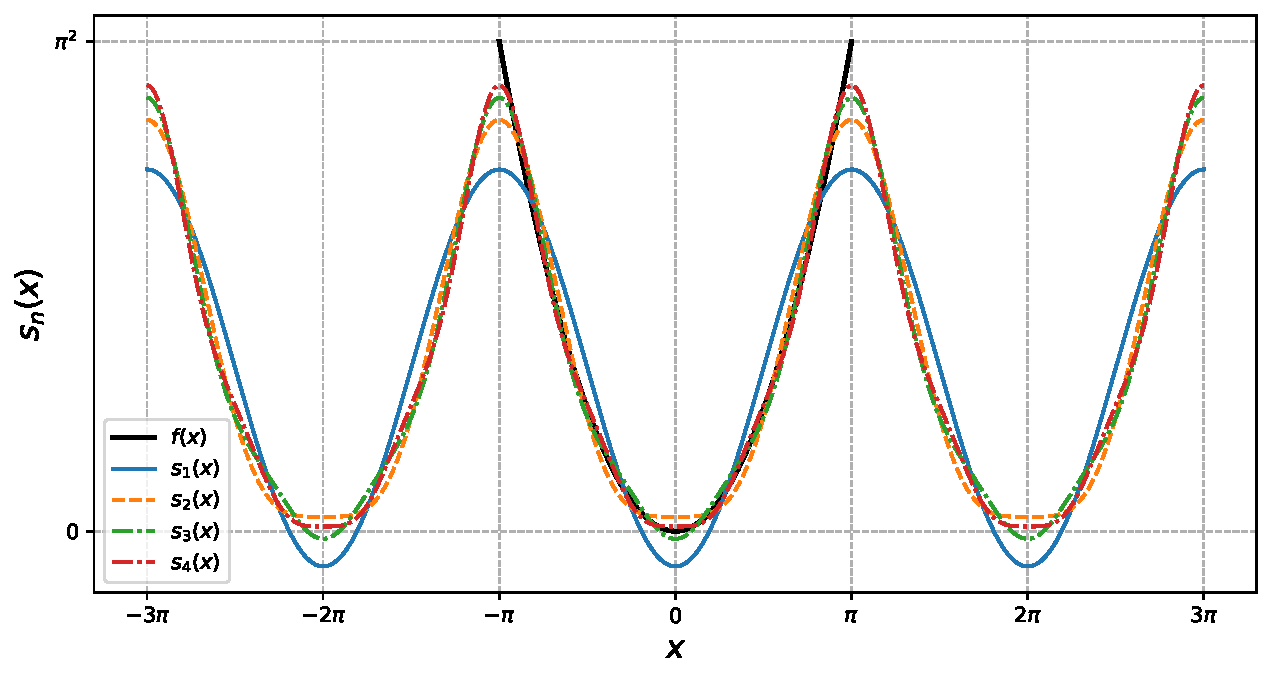
\includegraphics[scale = 0.65]{Figuras/EjemploFourier1.pdf}
    \caption{Serie de Fourier de la función $f(x) = x^2, -\pi \leq x \leq \pi$, truncada hasta $n = 4$.}
    \label{fig:EjemploFourier1}
\end{figure}

El teorema visto para convergencia uniforme nos garantiza que esta serie converge uniformemente a $f(x) = x^2$ en $[-\pi,\pi]$, es más, al aplicar el criterio de M de Weierstrass a la serie, ésta converge para todo $x \in \mathbb{R}$, pues
$$\forall  x \in \mathbb{R}: ~ \left|(-1)^n \frac{4}{n^2} \cos(nx)\right| \leq \frac{4}{n^2} = M_n ~~\mbox{y}~~  \sum\limits_{n=1}^{\infty} M_n < \infty.$$

\end{ejemplo}

Podemos usar la expansión en serie de Fourier de $f(x) = x^2$ en $[-\pi,\pi]$ para probar que 
$$\sum_{n=1}^{\infty} \frac{1}{n^2} = 1 + \frac{1}{4} + \frac{1}{9} + \cdots = \frac{\pi^2}{6}.$$

En efecto, al evaluar $x = \pi$ en \eqref{FourierCuadratica}, obtenemos que 
$$f(\pi) = \frac{\pi^2}{3} + \sum_{n=1}^{\infty} (-1)^n \frac{4}{n^2} \cos(n\pi) = \frac{\pi^2}{3} + \sum_{n=1}^{\infty} (-1)^{2n} \frac{4}{n^2} = \frac{\pi^2}{3} +  \sum_{n=1}^{\infty} \frac{4}{n^2}.$$

Así,
$$\pi^2 = \frac{\pi^2}{3} + 4 \sum_{n=1}^{\infty} \frac{1}{n^2} \Rightarrow \sum_{n=1}^{\infty} \frac{1}{n^2} = \frac{\pi^2}{6}.$$

\begin{ejemplo} \label{Signo}
Consideremos la función signo  definida por
$$f(x) := \left\{ \begin{array}{cc}
     -1,& - \pi \leq x < 0  \\
     1,&   0 \leq x \leq \pi
\end{array} \right. .$$

La función es seccionalmente continua con $x = 0$ punto de discontinuidad de salto y las derivadas laterales existen para todo $x \in (-\pi,\pi)$, luego la serie de Fourier de $f$ converge puntualmente a $f$ en los puntos de continuidad y a 
$$\frac{f(0^-) + f(0^+)}{2} = 0, \quad \mbox{en} ~ x = 0 ~~\mbox{y}$$
$$\frac{f(-\pi^+) + f(\pi^-)}{2} = 0, \quad \mbox{en} ~ x = \pm \pi. $$

Sus coeficientes de Fourier están dados por:
\begin{align*}
    a_0 &= \frac{1}{\pi} \int_{-\pi}^{\pi} f(x) \,dx = 0 , \\
    a_n &= \frac{1}{\pi} \int_{-\pi}^{\pi} f(x) \cos(n x)\,dx = 0, \quad n = 1,2,\dots
\end{align*}
\begin{align*}
     b_n &= \frac{1}{\pi} \int_{-\pi}^{\pi} f(x) \sin(nx) \,dx \\
     &= \frac{1}{\pi} \int_{-\pi}^0 (-1) \sin(nx)\,dx + \frac{1}{\pi} \int_{0}^{\pi} (1) \sin(nx) \,dx \\
     &= \left.  \frac{1}{\pi n} \cos(nx) \right|_{-\pi}^0 - \left. \frac{1}{\pi n} \cos(nx) \right|_{0}^{\pi} \\
     &= \frac{2}{\pi n} [1 - (-1)^n] \\
     &= \left\{ \begin{array}{cl}
         0, & n ~\mbox{par}  \\
         \frac{4}{\pi n}, &  n ~\mbox{impar}
     \end{array} \right. .
\end{align*}

Entonces, su serie de Fourier es 
$$f(x) =  \sum_{n ~impar} \frac{4}{\pi n} \sin(nx) = \sum_{k=1}^{\infty} \frac{4}{\pi} \frac{\sin[(2k-1)x]}{ (2k-1)}.$$

\textbf{Aclaración:} Note que a pesar de haber escrito que la función $f$ es igual a la serie, debemos tener en cuenta que en los punto $x = 0$ y $x = \pm \pi$ converge al valor medio del salto de la discontinuidad.

Es claro que la serie de Fourier de $f$ para todo $x\in \mathbb{R}$ representa la extensión periódica de los valores de $f(x)$ en el intervalo $[-\pi,\pi]$.

La gráfica de $f$ en conjunto con diferentes sumas parciales de su serie de Fourier están representadas en la figura \ref{fig:EjemploFourier2}.

\begin{figure}[H]
    \centering
    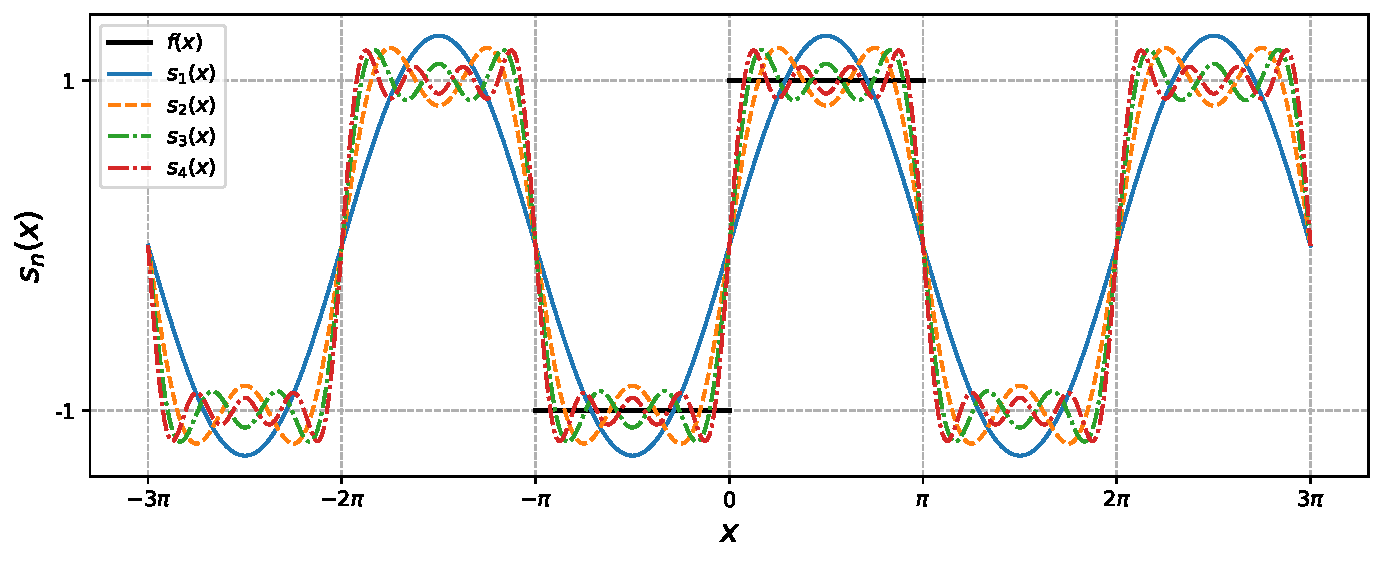
\includegraphics[scale = 0.65]{Figuras/EjemploFourier2.pdf}
    \caption{Serie de Fourier de la función signo truncada hasta $n = 4$.}
     \label{fig:EjemploFourier2}
\end{figure}

\end{ejemplo}

\section{Serie exponencial}

En el espacio $\mathcal{C}[-\pi,\pi]$ consideremos el sistema ortonormal completo 
$$\left\{ \frac{1}{\sqrt{2\pi}} e^{int} \right\}_{n= - \infty}^{n = \infty}$$

llamado \textbf{sistema exponencial}.

\begin{defi}
Sea $f \in \mathcal{C}[-\pi,\pi]$, la serie 
\begin{equation}
     \sum_{n=- \infty}^{\infty} c_n e^{int} \label{FourierExpo}
\end{equation}

se denomina \textbf{serie exponencial de Fourier}  donde los \textit{coeficientes de Fourier} están dados por:
\begin{equation*}
    c_n = \frac{1}{2\pi} \int_{-\pi}^{\pi} f(t) e^{-int} \,dt.
\end{equation*}
\end{defi}

\textbf{Observación}: La serie de Fourier de $f$ converge en media a $f$, o sea, 
\begin{shaded}
 $$f(t) \sim \sum_{n=- \infty}^{\infty} c_n e^{int}.$$   
\end{shaded}

\begin{propo} \label{TrigoExpo}
La $n$-ésima suma parcial de la serie de Fourier trigonométrica de una función (real o compleja) es igual a la $n$-ésima suma parcial de la serie exponencial.
\end{propo}

\begin{demo}
La $n$-ésima suma parcial de la serie exponencial es
$$ s_n(t) = \sum_{k=-n}^n c_k e^{ikt}.$$

Separando la suma:
\begin{align*}
    s_n(t) &= \sum_{k=-n}^{-1} c_k e^{ikt} + c_0 + \sum_{k=1}^n c_k e^{ikt} \\
    &= c_0 + \sum_{k=1}^n c_k e^{ikt} + \sum_{k=1}^n c_{-k} e^{-ikt} \\
    &= c_0 + \sum_{k=1}^n [c_k e^{ikt} + c_{-k} e^{-ikt}]. 
\end{align*}

Usando la identidad de Euler, $e^{i\theta} = \cos(\theta) + i \sin(\theta)$, encontramos que
$$s_n(t) = c_0 +  \sum_{k=1}^n [(c_k + c_{-k}) \cos(kt) + i(c_k - c_{-k}) \sin(kt)].$$

Desarrollando los coeficientes de la serie exponencial de Fourier, tenemos que
\begin{align*}
    c_0 &= \frac{1}{2\pi} \int_{-\pi}^{\pi} f(t) \,dt, \\
    c_k + c_{-k} &= \frac{1}{2\pi} \int_{-\pi}^{\pi} f(t) e^{-ikt} \,dt + \frac{1}{2\pi} \int_{-\pi}^{\pi} f(t) e^{ikt} \,dt  \\
    &= \frac{1}{2\pi} \int_{-\pi}^{\pi} f(t) [e^{ikt} + e^{-ikt}] \,dt \\
    &= \frac{1}{\pi} \int_{-\pi}^{\pi} f(t) \cos(kt) \,dt; \quad k = 1,2, \dots\\
   i( c_k - c_{-k}) &= \frac{i}{2\pi} \int_{-\pi}^{\pi} f(t) e^{-ikt} \,dt - \frac{i}{2\pi} \int_{-\pi}^{\pi} f(t) e^{ikt} \,dt \\
   &= - \frac{i}{2\pi} \int_{-\pi}^{\pi} f(t) [e^{ikt} - e^{-ikt}] \,dt \\
   &= \frac{1}{\pi} \int_{-\pi}^{\pi} f(t) \sin(kt)\,dt; \quad k = 1,2, \dots
\end{align*}

Comparando las expresiones obtenidas con los coeficientes de la serie de Fourier trigonométrica, podemos concluir que 
$$c_0 = \frac{a_0}{2}, ~  c_k + c_{-k} = a_k, ~ i( c_k - c_{-k}) = b_k; \quad k = 1,2, \dots$$

Por lo tanto, 
$$ s_n(t) = \sum_{k=-n}^n c_k e^{ikt} = \frac{a_0}{2} + \sum_{k=1}^n (a_k \cos(kt) + b_k \sin(kt)).$$

\end{demo}

\textbf{Observación 1:} Una consecuencia inmediata de la proposición \ref{TrigoExpo} es que todos los teoremas vistos para la serie de Fourier trigonométrica son aplicables a la serie de Fourier exponencial.
\\

\textbf{Observación 2:} Los coeficientes de las series \eqref{FourierTrigo} y \eqref{FourierExpo} están relacionados por 
\begin{equation}
a_0 = 2c_0,~~ a_n = c_n + c_{-n}, ~~ b_n = i(c_n - c_{-n}); \quad n = 1,2, \dots    \label{RelacionCoefi1}
\end{equation}

o bien, 
\begin{equation}
    c_n = \left\{ \begin{array}{cl}
        \frac{1}{2} (a_n - ib_n), & n \geq 0  \\
    \frac{1}{2}(a_{-n} + i b_{-n}),     & n  \leq -1 
    \end{array} \right. . \label{RelacionCoefi2}
\end{equation}

Si $f(t)$ es una función real, entonces sus respectivos coeficientes complejos $c_n$ satisfacen la relación:
$$c_n^* = \frac{1}{2\pi} \int_{-\pi}^{\pi} f(t) (e^{-int})^* \,dt = \frac{1}{2\pi} \int_{-\pi}^{\pi} f(t) e^{int} \,dt = c_{-n}.$$

\section{Diferenciación e integración de las series de Fourier}

Supongamos que tenemos una serie de funciones
$$\sum_{n=1}^{\infty} f_n(t),$$

y queremos integrarla (o derivarla). Resulta tentador intercambiar la integral (o derivada) por la serie, es decir, integrar (o derivar) término a término. Sin embargo, este intercambio no es siempre posible porque puede romper la convergencia de la serie. Por ejemplo, las series de potencia se pueden integrar (o derivar) término a término en su región de convergencia sin problema. En nuestro caso, nos interesa saber que condiciones deben cumplirse para las series de Fourier.

\begin{teorema}[Integración]
Sea $f$ una función seccionalmente continua en el intervalo $-\pi < t < \pi$. Independiente si la serie \eqref{FourierTrigo} converge, la siguiente ecuación es válida cuando $-\pi \leq t \leq \pi$:
\begin{equation*}
  \int_{-\pi}^t f(s) \,ds = \frac{a_0}{2} (t + \pi) + \sum_{n=1}^{\infty} \frac{1}{n} \left\{ a_n \sin(nt) - b_n[\cos(nt) + (-1)^{n+1}] \right\}.   
\end{equation*}
\end{teorema}

\begin{demo}
Consultar la sección \ref{DemostracionesFourier}.
\end{demo}

\begin{teorema}[Derivación]
Sea $f$ una función continua en $[-\pi,\pi]$, donde $f(-\pi) = f(\pi)$, y $f'$ es seccionalmente continua en el intervalo $(-\pi,\pi)$. Entonces, la serie de Fourier
\begin{equation*}
    f(t) = \frac{a_0}{2} + \sum_{n=1}^{\infty} (a_n \cos(nt) + b_n \sin (nt) ), \quad t \in [-\pi,\pi],
\end{equation*}

donde 
$$a_n = \frac{1}{\pi} \int_{-\pi}^{\pi} f(t) \cos(nt) \,dt, \quad b_n = \frac{1}{\pi} \int_{-\pi}^{\pi} f(t) \sin(nt) \,dt,$$

es derivable para todo $t \in (-\pi,\pi)$ en el cual $f''(t)$ existe:
\begin{equation*}
    f'(t) = \sum_{n=1}^{\infty} (- n a_n \sin(nt) + nb_n \cos(nt)).
\end{equation*}
\end{teorema}

\begin{demo}
Consultar la sección \ref{DemostracionesFourier}.
\end{demo}

\begin{ejemplo}
Obtener el desarrollo en serie de Fourier de la función $x^3$ en el intervalo $[-\pi,\pi]$.
\\

\textbf{Solución}: Las funciones del tipo $x^n$, $n \in \mathbb{N}$ son continuas, derivables e integrables, por lo que podemos aplicar estas operaciones a las series de Fourier que se obtengan a partir de ellas.  En nuestro caso obtendremos el desarrollo de $x^3$ por integración de $x^2$, cuyo desarrollo en serie de Fourier ya obtuvimos en el ejemplo \ref{EjemploFourier1}:
\begin{align*}
   \forall x \in [-\pi,\pi]:  \int_{-\pi}^x t^2 \,dt &=   \int_{-\pi}^x   \frac{\pi^2}{3} + \sum_{n=1}^{\infty} (-1)^n \frac{4}{n^2} \cos(nt) \,dt\\
    \Rightarrow ~ \frac{x^3}{3} + \frac{\pi^3}{3} &=  \frac{\pi^2}{3} (x+\pi) + \sum_{n=1}^{\infty} (-1)^n \frac{4 }{n^3}  \sin(nx)  \\
\Rightarrow \qquad \quad    x^3 &= \pi^2 x + 12 \sum_{n=1}^{\infty} \frac{(-1)^n}{n^3} \sin(nx).
\end{align*}

Lo que obtuvimos es el desarrollo en serie de $x^3-\pi^2 x$. Para obtener el desarrollo de $x^3$, encontremos la serie de Fourier de $x$, para ello utilicemos el desarrollo de $x^2$, pero esta vez derivando:
\begin{align*}
    \frac{d}{dx} [x^2] &= \frac{d}{dx} \left[  \frac{\pi^2}{3} + \sum_{n=1}^{\infty} (-1)^n \frac{4}{n^2} \cos(nx)\right] \\
   \Rightarrow \qquad 2x &= - \sum_{n=1}^{\infty} (-1)^n \frac{4}{n} \sin(nx) \\
   \Rightarrow \qquad ~ x &= - 2 \sum_{n=1}^{\infty}  \frac{(-1)^n}{n} \sin(nx).
\end{align*}

Sustituyendo en $x^3$:
\begin{align*}
    x^3 &= -2 \pi^2 \sum_{n=1}^{\infty}  \frac{(-1)^n}{n} \sin(nx) + 12 \sum_{n=1}^{\infty} \frac{(-1)^n}{n^3} \sin(nx) \\
    &= \sum_{n=1}^{\infty} \frac{(-1)^n}{n^3} \left[ 12 - 2\pi^2 n^2 \right] \sin(nx).
\end{align*}
\end{ejemplo}

\section{Fenómeno de Gibbs}

Cuando queremos aproximar una función $f$ con las sumas parciales de su serie de Fourier, se puede observar un comportamiento particular cerca de los puntos de discontinuidad aislados, por ejemplo, al graficar la serie de Fourier de la función signo para un $n$ alto, ver figura \ref{fig:GibssSign}, se comete un error considerable en las cercanías al punto de discontinuidad, y además este
error no disminuye si se incluyen más términos en la serie. Este efecto indeseado se denomina \textbf{fenómeno de Gibbs}. 

\begin{figure}[H]
    \centering 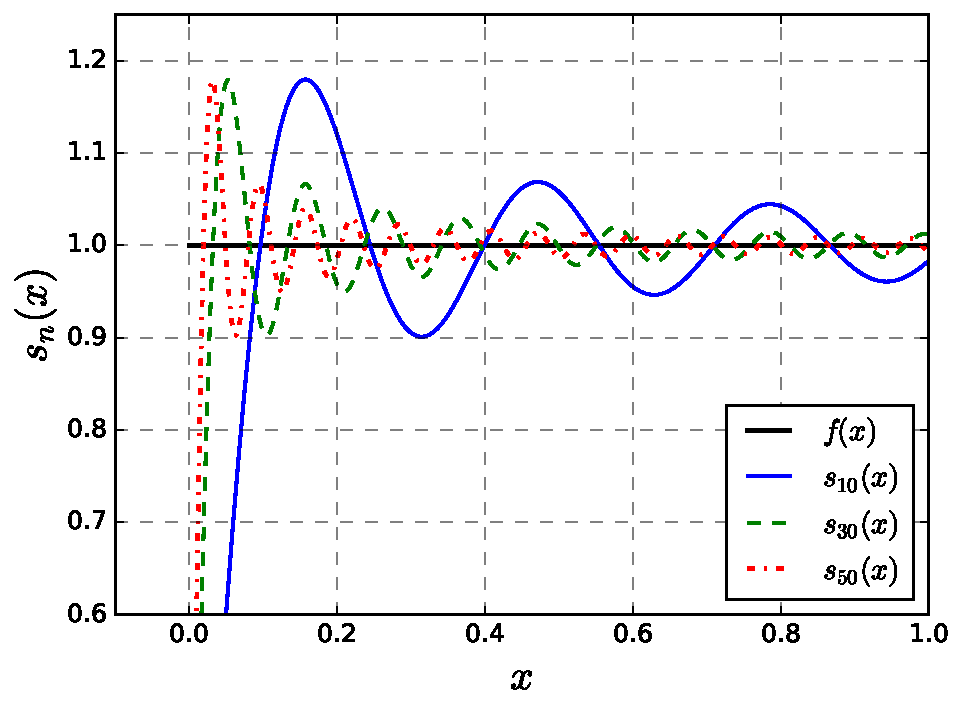
\includegraphics[scale = 0.65]{Figuras/FenomenoGibbs.pdf}
    \caption{Fenómeno de Gibbs en la función signo para $n = 10,30,50$.}
    \label{fig:GibssSign}
\end{figure}

Ilustremos este hecho con un análisis analítico de la función ya estudiada
$$f(x) = \left\{ \begin{array}{cc}
     -1,& - \pi \leq x < 0  \\
     1,&   0 \leq x \leq \pi
\end{array} \right. .$$

Su serie de Fourier está dada por
$$\sum_{n=1}^{\infty} \frac{4}{\pi} \frac{\sin[(2n-1)x]}{ (2n-1)}.$$

Sea 
$$s_n(x) = \frac{4}{\pi} \sum_{k=1}^n \frac{\sin[(2k-1)x]}{2k-1}$$

su $n$-ésima suma parcial. Derivando y multiplicando por $\pi \sin(x)$, encontramos que 
\begin{align*}
   \pi (\sin x)s_n'(x) =4 \sin(x) \sum_{k=1}^n \cos[(2k-1)x] &= 4 \sum_{k=1}^n   \sin(x) \cos[(2k-1)x] \\
   &= 4 \sum_{k=1}^n  \frac{1}{2}[\sin(x + (2k-1)x) + \sin(x - (2k-1)x)] \\
   &= 2 \sum_{k=1}^n [\sin(2k x) - \sin([2k-2]x)] \\
   &= 2 \sin(2nx).
\end{align*}

Luego, 
\begin{equation*}
  2 \sin(2nx_c) = 0 ~\Leftrightarrow~ x_c = \frac{m \pi}{2n}, \quad m \in \mathbb{Z}. 
\end{equation*}

Nos interesa encontrar el primer máximo de $s_n(x)$, así que tomaremos los valores $m = \pm 1$ de prueba, pues en $m = 0$ no se alcanza un máximo dado que $s_n(0) = 0$. Como $\sin(x_c) \neq 0$, para estos valores de $m$,  $s_n'(x_c) = 0$ y, en consecuencia, $x_c$ son los puntos críticos de $s_n$. 

En la siguiente tabla se analizan los signos de $s_n'(x)$.

\begin{figure}[H]
    \centering
    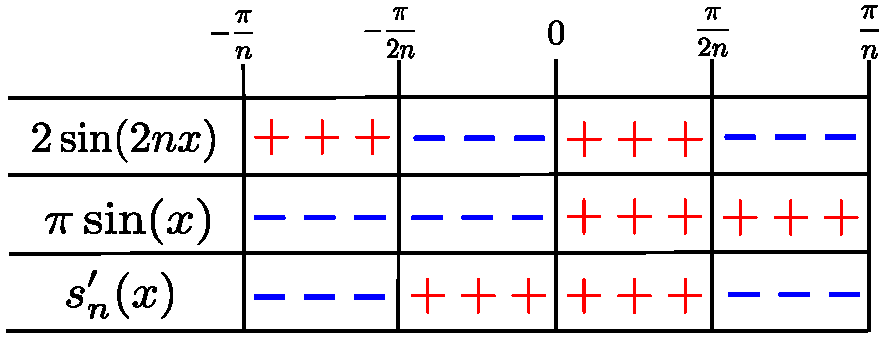
\includegraphics[scale = 0.62]{Figuras/EjemploGibbs.pdf}
    \caption{Tabla con el análisis de signos de $s_n'(x)$ asociada a la función signo.}
\end{figure}

Por el criterio de la primera derivada, vemos que $s_n$ tiene un máximo en $x_n = \frac{\pi}{2n}$. El valor de ese máximo es
$$s_n \left( \frac{\pi}{2n}\right) = \frac{4}{\pi} \sum_{k=1}^n \frac{\sin[(2k-1)\pi/2n]}{2k-1} = \frac{2}{\pi} \sum_{k=1}^n \frac{\sin[(2k-1)\pi /2n]}{(2k-1) \pi/2n} \left(\frac{\pi}{n} \right).$$

Notemos que la sumatoria 
$$ \sum_{k=1}^n \frac{\sin[(2k-1)\pi /2n]}{(2k-1) \pi/2n} \left(\frac{\pi}{n} \right)$$

es una suma de Riemann para la función $\sin y/y$ en $[0,\pi]$ para la partición regular $0 = x_0 < x_1  <  \cdots< x_n =  \pi$ con $x_i = (\pi/n) i$, $i = 0,1, \dots, n$ y eligiendo el punto medio de cada intervalo $[x_{k-1},x_k]$,
$$ \frac{x_{k-1} + x_k}{2} = (2k-1) \frac{\pi}{2n}, \quad  k = 1, \dots, n,$$

para evaluar $\sin y/y$. Entonces, 
$$\int_0^{\pi} \frac{\sin y}{y} \,dy \approx \frac{\pi}{2} s_n\left( \frac{\pi}{2n}\right).$$

Como 
$$\int_0^{\pi} \frac{\sin y}{y} \,dy ~~ \mbox{converge} ~\Rightarrow~ \lim_{n \to + \infty} s_n\left( \frac{\pi}{2n} \right) = \frac{2}{\pi} \int_0^{\pi} \frac{\sin y}{y} \,dy.$$

Usando un método numérico de integración (o su calculadora de integrales favorita), se tiene que 
$$\int_0^{\pi} \frac{\sin y}{y} \,dy \approx 1.85193\dots$$

Por lo tanto, 
$$\lim_{n \to + \infty} s_n\left( \frac{\pi}{2n} \right) \approx 1.179.$$

Así, las aproximaciones exceden el valor real de $f(0^+) = 1$ por $0.179$ o $8.95\%$ del salto de $f(0^-)$ a $f(0^+)$. 
\\

En general, se puede demostrar el siguiente teorema, debido a M. B$\hat{\mbox{o}}$cher \cite{Bôcher}:

\begin{teorema}
Sea $f$ una función de variable real, con período $2\pi$. Supongamos que $f$ y $f'$ son ambas continuas excepto para un número finito de discontinuidades de salto en el intervalo $[-\pi,\pi]$. Sea $s_n(x)$ la suma parcial de orden $n$ de Fourier. Entonces, en un punto $a$ de discontinuidad, las gráficas de las funciones $s_n(x)$ convergen al segmento vectical (ver figura \ref{Gibbs}) de longitud 
$$L = \frac{2}{\pi} Si(\pi) |f(a^+) - f(a^-)| \approx 1.179 |f(a^+) - f(a^-)|$$

centrada en el punto 
$$\left(a, \frac{f(a^+) + f(a^-)}{2} \right),$$

donde 
$$Si(x) = \int_0^x \frac{\sin t}{t} \,dt$$

es la función seno integral.
\end{teorema}

\begin{figure}[H]
    \centering
    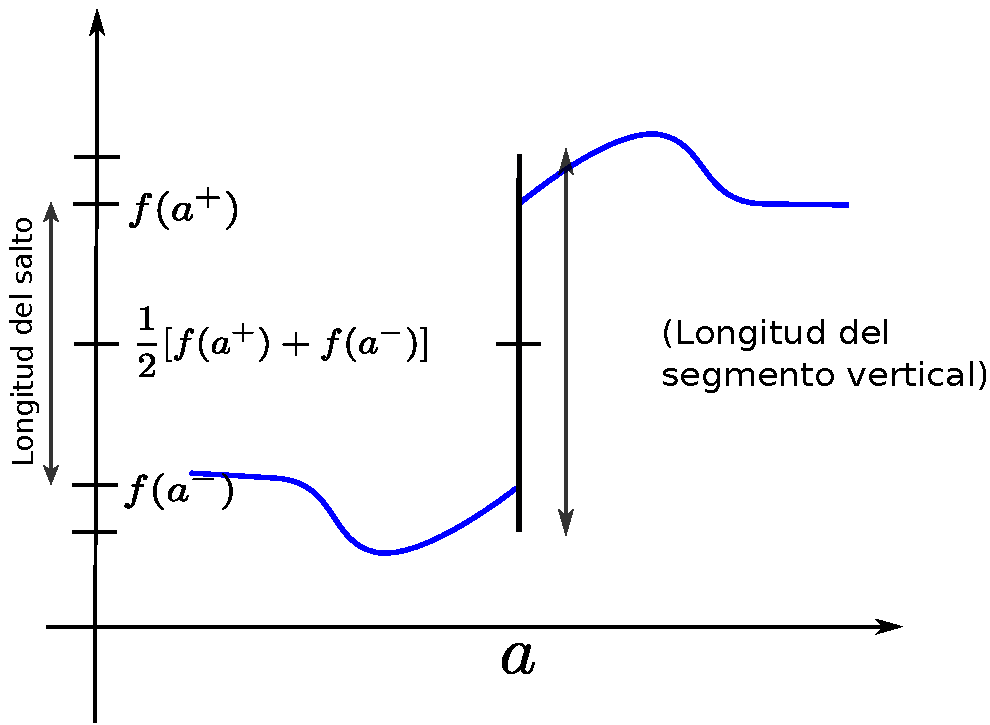
\includegraphics[scale = 0.55]{Figuras/Gibbs.pdf}
    \caption{Fenómeno de Gibbs en un punto de discontinuidad. Adaptado de \cite{UFRO}, pág. 202.}
    \label{Gibbs}
\end{figure}
 
\section{Cambio de intervalo}

Hasta ahora hemos estudiado funciones en el intervalo $[-\pi,\pi]$, sin embargo, es posible extender los resultados al caso de funciones seccionalmente continuas en un intervalo más general $[a,b]$. 

Sea $f \in \mathcal{C}[a,b]$, consideremos $\alpha: [- \pi,\pi] \longrightarrow [a,b]$ definida por \footnote{El lector puede llegar a esta función calculando la ecuación de la recta que pasa por los puntos $(-\pi,a)$ y $(\pi,b)$. La función resultante mapea biunívocamente los puntos del intervalo $[-\pi,\pi]$ a $[a,b]$.} 
$$\alpha(t) = a + \frac{b-a}{2\pi} (t+\pi)$$

la cual es continua, creciente con $\alpha(-\pi) = a$ y $\alpha(\pi) = b$. Ahora, si consideramos la función compuesta $g = f \circ \alpha$, se tiene que $g \in \mathcal{C}[-\pi,\pi]$. Luego, 
$$g(t) \sim \sum_{n= - \infty}^{\infty} c_n e^{int}$$

donde 
$$c_n = \frac{1}{2\pi} \int_{-\pi}^{\pi} g(t) e^{-int} \,dt, \quad n \in \mathbb{Z}.$$

Al hacer 
$$x = a + \frac{b-a}{2\pi} (t+\pi) ~\Leftrightarrow~ t = \frac{2x-b-a}{b-a} \pi = \frac{2 \pi}{b-a} x - \frac{b+a}{b-a} \pi  ,$$

se obtiene $g(t) = f(a + \frac{b-a}{2\pi} (t+\pi)) = f(x)$ y así 
$$f(x) \sim \sum_{n=-\infty}^{\infty} c_n \left[ e^{i\frac{2n\pi}{b-a} x} e^{-i \frac{b+a}{b-a}n\pi}\right].$$

Haciendo el cambio de variable $t = \frac{2\pi}{b-a} x - \frac{b+a}{b-a} \pi ~\Rightarrow~ dt = \frac{2\pi}{b-a} dx$, se obtiene
\begin{align*}
 c_n = \frac{1}{2\pi} \int_{-\pi}^{\pi} f(a + \frac{b-a}{2\pi} (t+\pi)) e^{-int} \,dt   &= \frac{1}{b-a} \int_a^b f(x) \left[ e^{-i\frac{2n\pi}{b-a} x} e^{i \frac{b+a}{b-a}n\pi}\right] \,dx \\
 &= \frac{1}{b-a} e^{i \frac{b+a}{b-a}n\pi} \int_a^b f(x) e^{-i \frac{2n\pi}{b-a}} \,dx.
\end{align*}

Por lo tanto, la serie de Fourier exponencial asociada a $f$ está dada por 
$$f(x) \sim \sum_{n=-\infty}^{\infty} f_n e^{i \frac{2n\pi}{b-a}x} $$

donde 
$$f_n = \frac{1}{b-a} \int_a^b f(x) e^{-i \frac{2n\pi}{b-a}} \,dx.$$

Si $f:[a,b] \longrightarrow \mathbb{C}$ se extiende periódicamente con período $T = b-a$ y definimos la \textbf{frecuencia fundamental} $\omega_1 := 2\pi/T$ y las \textbf{frecuencias armónicas} $\omega_n := n \omega_1, n = 0, \pm 1, \pm 2,\dots$ Entonces, la serie de Fourier exponencial puede escribirse como 
\begin{shaded}
  $$f(x) \sim \sum_{n = - \infty}^{\infty} f_n e^{i \omega_n x}$$
\end{shaded}

donde 
\begin{shaded}
$$f_n = \frac{1}{T} \int_a^b f(x) e^{-i \omega_n x} \,dx, \quad n = 0, \pm 1, \pm 2, \dots$$    
\end{shaded}

Usando las relaciones entre los coeficientes de la serie trigonométrica y la exponencial (vea \eqref{RelacionCoefi1}), se puede probar que la serie de Fourier trigonométrica para la función $f$, definida en los párrafos anteriores, es
\begin{shaded}
$$f(x) \sim \frac{a_0}{2} + \sum_{n=1}^{\infty} \left[a_n \cos(\omega_n x) + b_n \sin(\omega_n x) \right]$$    
\end{shaded}

con
\begin{shaded}
 \begin{align*}
    a_0 &= \frac{2}{T} \int_a^b f(x) \,dx , \\
    a_n &= \frac{2}{T} \int_a^b f(x) \cos(\omega_n x) \,dx; \quad n = 1,2 \dots \\
    b_n &= \frac{2}{T} \int_a^b f(x) \sin(\omega_n x) \,dx; \quad n = 1,2 \dots
\end{align*}   
\end{shaded}

\section{Demostraciones de teoremas} \label{DemostracionesFourier}

\subsection*{Convergencia puntual}

Antes de demostrar el teorema de la convergencia puntual, discutiremos dos lemas. El primero es un caso especial del conocido \textbf{lema de Riemann-Lebesgue}.

\begin{lema} \label{lema1}
Sea $g(u)$ una función seccionalmente continua en el intervalo $0 <u < \pi$. Entonces, 
\begin{equation}
    \lim_{n \to + \infty} \int_0^{\pi} g(u) \sin [(n + 1/2)u] \,du = 0 \label{LemaFourier1}
\end{equation}

donde $n$ es un entero positivo.
\end{lema}

\begin{demo}
Usando la identidad trigonométrica 
$$\sin(\alpha + \beta) = \sin \alpha \cos \beta + \cos \alpha \sin \beta,$$

tenemos que
\begin{align*}
    \int_0^{\pi} g(u) \sin [(n + 1/2)u] \,du &= \int_0^{\pi} g(u) \sin \left( \frac{u}{2} + n u\right) \,du \\
    &= \int_0^{\pi} g(u) \sin\left( \frac{u}{2}\right) \cos(nu) \,du + \int_0^{\pi} g(u) \cos \left( \frac{u}{2}\right) \sin(nu) \,du.
\end{align*}

Ahora, excepto por un factor de $2/\pi$, la primera de estas integrales es el coeficiente $a_n$ en la serie de Fourier de cosenos para la función seccionalmente continua $g(u) \sin(u/2)$ en el intervalo $0 < u < \pi$. La otra integral es, excepto por un factor de $2/\pi$, el coeficiente $b_n$ en la serie de Fourier de senos para la función seccionalmente continua $g(u) \cos(u/2)$ en el mismo intervalo. Por lo tanto, usando la proposición \ref{C.FourierCero}, el lema queda demostrado.
\end{demo}

\newpage

Nuestro segundo lema involucra el \textbf{núcleo de Dirichlet}:
  \begin{equation}
  \boxed{  D_n(u) = \frac{1}{2} + \sum_{k=1}^n \cos(ku), \quad n \in \mathbb{N}} \label{DirichletKernel}
\end{equation}  

Notemos que $D_n(u)$ es continuo, par y periódico con período $2\pi$. El núcleo de Dirichlet juega un importante papel en nuestra teoría y otras dos propiedades que nos serán útiles son:
\begin{align}
    \int_0^{\pi} D_n(u) \,du &= \frac{\pi}{2}, \label{DirichletKernel1} \\
    D_n(u) &= \frac{\sin[(n+1/2)u]}{2 \sin(u/2)}, \qquad u \neq 0, \pm 2\pi, \pm 4\pi, \dots \label{DirichletKernel2}
\end{align}

Es fácil de ver que la propiedad \eqref{DirichletKernel1} se cumple. Por otro lado, para verificar la propiedad \eqref{DirichletKernel2},  desarrollemos la expresión
$$ \sum_{k = -n}^{n} e^{i k u}.$$

Primero, efectuemos el cambio de índice $m = k + n$ de tal forma que el índice $m$ se mueva desde $m = 0$ hasta $m = 2n$.
$$ \sum_{k = -n}^{n} e^{i k u} = \sum_{m = 0}^{2n} e^{i(m-n)u} = e^{-inu} \sum_{m=0}^{2n}\left( e^{iu}\right)^m.$$

Reconocemos la suma de una progresión geométrica,
$$\sum_{k=0}^n r^k = \frac{1-r^{n+1}}{1-r},$$

con $r = e^{iu}, 0 < u < 2\pi$. Luego,
\begin{align*}
e^{-inu} \sum_{m=0}^{2n}\left( e^{iu}\right)^m &= e^{-inu} \frac{1-\left( e^{iu}\right)^{2n+1}}{1-e^{iu}} \textcolor{red}{\cdot \frac{e^{-iu/2}}{e^{-iu/2}}} \\
&= \frac{e^{-i(n + 1/2)u} - e^{i(n+1/2)u}}{e^{-iu/2} - e^{i u/2}} \\
&= \frac{-2i \sin[(n+1/2) u]}{-2i \sin(u/2)} \\
&=  \frac{\sin[(n+1/2) u]}{\sin(u/2)}.
\end{align*}

Ahora,
\begin{equation*}
     \sum_{k= -n}^{n} e^{i k u} = \sum_{k=-n}^{-1} e^{iku} + 1 + \sum_{k=1}^n e^{iku} = 1 + \sum_{k=1}^n [e^{iku} + e^{-iku}] = 1 + 2 \sum_{k=1}^n \cos(ku).
\end{equation*}

Entonces, 
\begin{shaded}
 \begin{equation}
 D_n(u) = \frac{1}{2} + \sum_{k=1}^n \cos(ku) = \frac{\sin[(n+1/2)u]}{2 \sin(u/2)}, \quad u \neq 0, \pm 2\pi, \pm 4\pi, \dots    \label{NucleoDirichlet}
\end{equation}   
\end{shaded}

\begin{lema} \label{lema2}
Supongamos que una función $g(u)$ es seccionalmente continua en el intervalo $0 < u < \pi$ y que la derivada por la derecha $g'(0^+)$ existe. Entonces,
\begin{equation}
    \lim_{n \to + \infty} \int_0^{\pi} g(u) D_n(u) \,du = \frac{\pi}{2} g(0^+), \label{LemaFourier2}
\end{equation}

donde $D_n(u)$ está definido por la ecuación \eqref{DirichletKernel}.
\end{lema}

\begin{demo}
Primero, escribamos 
\begin{equation}
    \int_0^{\pi} g(u) D_n(u) \,du = I_n + J_n, \label{LemaFourier3}
\end{equation}

donde 
$$I_n = \int_0^{\pi} [g(u) - g(0^+)] D_n(u) \,du ~~\mbox{y}~~ J_n = \int_0^{\pi} g(0^+) D_n(u) \,du.$$

Usando la expresión \eqref{DirichletKernel2}, la primera de estas dos integrales puede escribirse como 
\begin{equation}
   I_n = \int_0^{\pi} \frac{g(u) - g(0^+)}{2 \sin(u/2)} \sin [(n+1/2)u] \,du. \label{LemaFourier4}
\end{equation}

Observe que la función
$$G(u) =  \frac{g(u) - g(0^+)}{2 \sin(u/2)}$$

es el cociente de dos funciones seccionalmente continuas en el intervalo $0 < u <\pi$. Aunque el denominador se anule en $u = 0$, la existencia de g$g'(0^+)$ nos asegura la existencia de $G(0^+)$. En efecto,
$$\lim_{u \to 0^+} G(u) = \left( \lim_{u \to 0^+} \frac{g(u) - g(0^+)}{u-0} \right) \cancelto{1}{\left(\lim_{u \to 0^+} \frac{u/2}{\sin(u/2)}\right)}= g'(0^+).$$

Así $G(u)$ es seccionalmente continua en el intervalo $0<u<\pi$. Aplicando el lema \ref{lema1}, concluímos que
$$\lim_{n \to + \infty} I_n = 0.$$

Por otro lado, de la propiedad \eqref{DirichletKernel1} del núcleo de Dirichlet, tenemos que 
$$J_n = \frac{\pi}{2} g(0^+) ~\Rightarrow~ \lim_{n \to + \infty}J_n = \frac{\pi}{2} g(0^+).$$

Por lo tanto, tomando el límite cuando $n \to \infty$ en \eqref{LemaFourier3}:
$$\lim_{n \to + \infty}  \int_0^{\pi} g(u) D_n(u) \,du = \lim_{n \to + \infty} [I_n + J_n] = \frac{\pi}{2} g(0^+).$$
\end{demo}

\begin{teorema}[Convergencia puntual de la serie de Fourier] 
Sea $f(t)$ una función real seccionalmente continua en el intervalo $-\pi < t < \pi$. Su serie de Fourier trigonométrica converge al valor medio
\vspace{-0.05cm}
$$\frac{f(t^+) + f(t^-)}{2}$$

para cada $t \in (-\pi,\pi)$ donde ambas derivadas laterales $f'(t^+)$ y $f'(t^-)$ existen.
\end{teorema}

\begin{demo}
La $n$-ésima suma parcial de la serie de Fourier está dada por
\begin{align*}
    s_n(t) &= \frac{a_0}{2} + \sum_{k=1}^n (a_k \cos(kt) + b_k \sin(kt)) \\
    &= \frac{1}{2\pi} \int_{-\pi}^{\pi} f(x) \,dx + \frac{1}{\pi} \sum_{k=1}^n \left[ \int_{-\pi}^{\pi} f(x) \cos(k x) \,dx \cdot \cos(kt) + \int_{-\pi}^{\pi} f(x) \sin(k x) \,dx \cdot \sin(kt)\right] \\
    &= \frac{1}{\pi} \int_{-\pi}^{\pi} f(x) \left[\frac{1}{2} + \sum_{k=1}^n (\cos(kx) \cos(kt) + \sin(kx) \sin(kt)) \right] \,dx \\
    &= \frac{1}{\pi} \int_{-\pi}^{\pi} f(x) \left[ \frac{1}{2} + \sum_{k=1}^n \cos[k(x-t)] \right] \,dx.
\end{align*}

Usando la expresión del núcleo de Dirichlet dada por \eqref{DirichletKernel}:
$$s_n(t) = \frac{1}{\pi} \int_{-\pi}^{\pi} f(x) D_n(x-t) \,dx.$$

Haciendo la extensión periódica de $f$ a todo $\mathbb{R}$, 
$$f(x + 2\pi) = f(x), \quad \forall x \in \mathbb{R},$$

 resulta
 \begin{equation}
    s_n(t) = \frac{1}{\pi} \int_{t-\pi}^{t + \pi} f(x) D_n(x-t) \,dx,\label{Lema2.1}
 \end{equation}
 
donde el punto $t$ está en el centro del intervalo que escogimos. Ahora se sigue de la ecuación  \eqref{Lema2.1} que
\begin{equation}
  s_n(t) = \frac{1}{\pi} [I_n(t) + J_n(t)] \label{Lema2.2} 
\end{equation}

donde  
\begin{align}
    I_n(t) &= \int_{t}^{t+\pi} f(x) D_n(x-t) \,dx, \label{Lema2.3} \\
    J_n(t) &= \int_{t-\pi}^t f(x) D_n(x-t) \,dx. \label{Lema2.4} 
\end{align}

Haciendo el cambio de variable $u = x-t ~\Rightarrow~ du = dx $ en la integral \eqref{Lema2.3}, se obtiene
\begin{equation}
    I_n(t) = \int_{0}^{\pi} f(t+u) D_n(u) \,du.\label{Lema2.5} 
\end{equation}

Del hecho que $f$ sea seccionalmente continua en $(-\pi,\pi)$ y periódica (por la extensión hecha), ésta es seccionalmente continua en cualquier intervalo cerrado del eje $t$. Así que, para un valor arreglado de $t$, la función $g(u) = f(t+u)$ en \eqref{Lema2.5} es seccionalmente continua en cualquier intervalo cerrado del eje $u$, en particular $0<u<\pi$. Supongamos que que $f'(t^+)$ existe. Después de observar que
$$g(0^+) = \lim_{u \to 0^+} g(u) = \lim_{u \to 0^+} f(t+u) \overset{\textcolor{blue}{v = t+u}}{=} \lim_{v \to t^+} f(v) = f(t^+),$$

podemos mostrar que la derivada a la derecha de $g$ en  $u = 0$ existe:
\begin{equation*}
    g'(0^+) = \lim_{u \to 0^+} \frac{g(u) - g(0^+)}{u-0} = \lim_{u \to 0^+} \frac{f(t+u) - f(t^+)}{u} = f'(t^+).
\end{equation*}

De acuerdo al lema \ref{lema2}, tenemos que 
\begin{equation}
\lim_{n \to + \infty} I_n(t) = \frac{\pi}{2} g(0^+) = \frac{\pi}{2} f(t^+).    \label{Lema2.6}
\end{equation}

Por otro lado, haciendo la sustitución $u = t-x ~\Rightarrow~ du = -dx$ en la integral \eqref{Lema2.4} y recordando que $D_n(u)$ es par, obtenemos que
\begin{equation}
    J_n(t) = \int_0^{\pi} f(t-u) D_n(u) \,du. \label{Lema2.7}
\end{equation}

Ahora, asumimos que la derivada por la izquierda $f'(t^-)$ existe, y notemos que la función $g(u) = f(t-u)$ en la expresión \eqref{Lema2.7} es seccionalmente continua en el intervalo $0<u<\pi$. Más aún, 
$$g(0^+) = \lim_{u \to 0^+} g(u) = \lim_{u \to 0^+} f(t - u) = \lim_{v \to t^-} f(v) = f(t^-)$$

y
\begin{align*}
g'(0^+) = \lim_{u \to 0^+} \frac{g(u) - g(0^+)}{u-0} &= \lim_{u \to 0^+} \frac{f(t-u) - f(t^-)}{u} \\
&=   - \lim_{h \to 0^-} \frac{f(t+h) - f(t^-)}{h} \quad \textcolor{blue}{(h = -u)}\\
&= -f'(t^-).   
\end{align*}

Así que una vez más, por el lema \ref{lema2}, 
\begin{equation}
\lim_{n \to + \infty} J_n(t) = \frac{\pi}{2} g(0^+) = \frac{\pi}{2} f(t^-).    \label{Lema2.8}
\end{equation}

Finalmente, concluimos a partir de la ecuación \eqref{Lema2.2} y los límites \eqref{Lema2.6} y \eqref{Lema2.8} que 
$$\lim_{n \to + \infty} s_n(t) = \frac{f(t^+) + f(t^-)}{2}, \quad t \in (-\pi,\pi)$$

demostrando así el teorema.
\end{demo}

\subsection*{Convergencia uniforme}

\begin{teorema}[Convergencia uniforme] 
Supóngase que $f$ es continua en $[-\pi,\pi]$, $f(-\pi) = f(\pi)$ y que $f'$ es continua por tramos, con discontinuidades de salto. Entonces la serie de Fourier trigonométrica de $f$ converge a $f$ absolutamente y uniformemente.
\end{teorema}


\begin{demo}
Por el teorema \ref{Puntual}, podemos escribir
$$f(t) = \frac{a_0}{2} + \sum_{n=1}^{\infty}(a_n \cos(nt) + b_n \sin(nt)), \quad t \in [-\pi,\pi].$$

Los coeficientes de Fourier de $f'$ son 
$$\alpha_n = \frac{1}{\pi} \int_{-\pi}^{\pi} f'(t) \cos(nt) \,dt, \quad \beta_n = \frac{1}{\pi} \int_{-\pi}^{\pi} f'(t) \sin(nt) \,dt.$$

Luego,
$$\alpha_n = \left. \frac{1}{\pi} f(t) \cos(nt) \right|_{-\pi}^{\pi} + \frac{n}{\pi} \int_{-\pi}^{\pi} f(t) \sin(nt) \,dt = n b_n, $$

ya que podemos integrar por partes y $f(\pi) = f(-\pi)$. Análogamente, $\beta_n = - na_n$.

Por lo tanto, 
$$a_n = - \frac{\beta_n}{n}, ~~ b_n = \frac{\alpha_n}{n}, \quad n = 1,2, \dots$$

Sabemos que $\sum\limits_{n=1}^{\infty} \beta_n^2$ converge por la desigualdad de Bessel para $f'$. Sea $s_n = \sum\limits_{k=1}^n |a_k|$,
$$s_n = \sum_{k=1}^n \frac{|\beta_k|}{k}  \leq \left\{ \left( \sum_{k=1}^n  \beta^2_k \right) \left(\sum_{k=1}^n \frac{1}{k^2} \right) \right\}^{1/2} \leq \left\{ \left( \sum_{k=1}^{\infty}  \beta^2_k \right) \left(\sum_{k=1}^{\infty}  \frac{1}{k^2} \right) \right\}^{1/2}  $$

por la desigualdad de Cauchy-Schwarz para $\mathbb{R}^n$. 

Como $s_n$ es una sucesión de términos no negativos y está acotada, la serie
\begin{equation}
    \sum_{n=1}^{\infty} |a_n| < \infty. \label{uniforme1}
\end{equation}

De manera similar se prueba que 
\begin{equation}
    \sum_{n=1}^{\infty} |b_n| < \infty. \label{uniforme2}
\end{equation}

Como $\alpha_n, \beta_n \to 0$ (consecuencia de la desigualdad de Bessel), también tenemos que  
$$\lim_{n \to \infty} n a_n = \lim_{n \to \infty} n b_n = 0.$$

Ahora solo basta mostrar que 
$$\frac{a_0}{2} + \sum_{n=1}^{\infty}(a_n \cos(nt) + b_n \sin(nt))$$

converge uniformemente, ya que el límite debe ser $f(t)$. A su vez, basta mostrar que 
$$\sum_{n=1}^{\infty} (a_n \cos(nt) + b_n \sin(nt))$$

es uniformemente convergente. Pero,
$$|a_n \cos(nt) + b_n \sin(nt)| \leq |a_n| + |b_n| = M_n,$$

y entonces, por \eqref{uniforme1} y \eqref{uniforme2}, la serie de términos no negativos $\sum\limits_{n=1}^{\infty} M_n$ converge.

Por lo tanto, por el criterio de M de Weierstrass, la serie converge uniforme y absolutamente.

\end{demo}

\subsection*{Diferenciación e integración}

\begin{teorema}[Integración]
Sea $f$ una función seccionalmente continua en el intervalo $-\pi < t < \pi$. Independiente si la serie \eqref{FourierTrigo} converge, la siguiente ecuación es válida cuando $-\pi \leq t \leq \pi$:
\begin{equation}
  \int_{-\pi}^t f(s) \,ds = \frac{a_0}{2} (t + \pi) + \sum_{n=1}^{\infty} \frac{1}{n} \left\{ a_n \sin(nt) - b_n[\cos(nt) + (-1)^{n+1}] \right\}.    \label{Integral}
\end{equation}
\end{teorema}

\begin{demo}
Nuestra demostración comienza con el hecho que, como $f$ es seccionalmente continua, la función
\begin{equation}
  F(t) = \int_{-\pi}^t f(s) \,ds - \frac{a_0}{2} t, \quad t \in [-\pi,\pi] \label{Integral1}
\end{equation}

es continua. Más aún, 
$$F'(t) = f(t) - \frac{a_0}{2}, \qquad - \pi < t <\pi, $$

excepto en los puntos donde $f$ es discontinua. Así, $F'$ es seccionalmente continua en el intervalo $(-\pi,\pi)$. Por lo tanto, $F$ tiene derivada seccionalmente continua (existen $F'(t^+)$ y $F'(t^-)$), entonces se sigue del teorema \eqref{Puntual} que
\begin{equation}
    F(t) = \frac{A_0}{2} + \sum_{n=1}^{\infty} (A_n \cos(nt) + B_n \sin(nt)), \quad t \in (-\pi,\pi), \label{Integral2}
\end{equation}

donde 
\begin{equation}
    A_n =  \frac{1}{\pi} \int_{-\pi}^{\pi} F(t) \cos(nt) \,dt, \quad B_n = \frac{1}{\pi} \int_{-\pi}^{\pi} F(t) \sin(nt) \,dt.\label{Integral3}
\end{equation}

Notemos de la expresión \eqref{Integral1} que 
$$F(\pi) = \int_{-\pi}^{\pi} f(s) \,ds - \frac{a_0}{2} \pi = a_0 \pi - \frac{a_0}{2}\pi = \frac{a_0}{2}\pi$$

y $F(-\pi) = \frac{a_0}{2}\pi$, luego $F(\pi) = F(- \pi)$. Ésto nos muestra que la representación \eqref{Integral2} es también valida en los extremos del intervalo $(-\pi,\pi)$ y, por lo tanto, en cada punto $x \in [-\pi,\pi]$.

Escribamos ahora los coeficientes $A_n$ y $B_n$ en términos de $a_n$ y $b_n$. Cuando $n \geq 1$, podemos integrar por partes las integrales \eqref{Integral3}, usando el hecho de que $F$ es continua y $F'$ seccionalmente continua. Entonces,
\begin{align*}
    A_n &= \frac{1}{n\pi} \cancelto{0}{[F(t) \sin(nt)]_{-\pi}^{\pi}} - \frac{1}{n\pi} \int_{-\pi}^{\pi} F'(t) \sin(nt) \,dt \\
    &=  - \frac{1}{n\pi} \int_{-\pi}^{\pi} \left[ f(t) - \frac{a_0}{2} \right] \sin(nt) \,dt \\
    &= - \frac{1}{n\pi} \int_{-\pi}^{\pi} f(t) \sin(nt) \,dt + \frac{a_0}{2n\pi} \int_{-\pi}^{\pi} \sin(nt) \,dt \\
    &= - \frac{b_n}{n} + \frac{a_0}{2n\pi} \cancelto{0}{\left[ -\frac{1}{n} \cos(nt)\right]_{-\pi}^{\pi} } = - \frac{b_n}{n}.
\end{align*}

Similarmente, $B_n = a_n/n$. Con respecto a $A_0$, sabemos que $F(\pi) = \frac{a_0}{2}\pi$ y que la representación \eqref{Integral2} es también válida cuando $x = \pi$. Así que, evaluando $t = \pi$ en la representación y luego resolviendo para $A_0$, vemos que
$$A_0 = a_0 \pi - 2 \sum_{n=1}^{\infty} (-1)^n A_n = a_0 \pi - 2 \sum_{n=1}^{\infty} \frac{(-1)^{n+1}}{n} b_n.$$

A partir del desarrollo de la demostración del teorema \ref{C.Uniforme}, probamos que 
$$\sum_{n=1}^{\infty} |(-1)^n A_n| = \sum_{n=1}^{\infty} |A_n| < \infty ~\Rightarrow~ \sum_{n=1}^{\infty} (-1)^n A_n < \infty.$$

Con las expresiones para $A_n$ y $B_n$, incluyendo la expresión en serie de $A_0$, la serie \eqref{Integral2} toma la forma 
$$F(t) = \frac{a_0}{2}\pi + \sum_{n=1}^{\infty} \frac{1}{n} \left\{ a_n \sin(nt) - b_n [\cos(nt) + (-1)^{n+1}] \right\}.$$

Finalmente, si sustituimos este resultado en  \eqref{Integral1}, llegamos al resultado deseado \eqref{Integral}.
\end{demo}

\begin{teorema}[Derivación]
Sea $f$ una función continua en $[-\pi,\pi]$, donde $f(-\pi) = f(\pi)$, y $f'$ es seccionalmente continua en el intervalo $(-\pi,\pi)$. Entonces, la serie de Fourier
\begin{equation}
    f(t) = \frac{a_0}{2} + \sum_{n=1}^{\infty} (a_n \cos(nt) + b_n \sin (nt) ), \quad t \in [-\pi,\pi], \label{Derivada1}
\end{equation}

donde 
$$a_n = \frac{1}{\pi} \int_{-\pi}^{\pi} f(t) \cos(nt) \,dt, \quad b_n = \frac{1}{\pi} \int_{-\pi}^{\pi} f(t) \sin(nt) \,dt,$$

es derivable para todo $x \in (-\pi,\pi)$ en el cual $f''(t)$ existe:
\begin{equation}
    f'(t) = \sum_{n=1}^{\infty} ( - n a_n \sin(nt) + nb_n \cos(nt)).\label{Derivada2}
\end{equation}
\end{teorema}

\begin{demo}
Sea $t \in (-\pi,\pi)$ un punto el cual $f''$ existe, luego $f'$ es continua en $t$. Así, aplicando el teorema \ref{Puntual} a la función $f'$, 
\begin{equation}
    f'(t) = \frac{\alpha_0}{2} + \sum_{n=1}^{\infty} (\alpha_n \cos(nt) + \beta_n \sin(nt)), \label{Derivada3}
\end{equation}

donde 
$$\alpha_n = \frac{1}{\pi} \int_{-\pi}^{\pi} f'(t) \cos(nt) \,dt, \quad \beta_n = \frac{1}{\pi} \int_{-\pi}^{\pi} f'(t) \sin(nt) \,dt.$$

Sin embargo, $f$ y $f'$ satisfacen las condiciones del teorema \eqref{C.Uniforme}, luego sabemos a partir de la demostración hecha que 
\begin{equation*}
    \alpha_0 = 0, \quad \alpha_n = n b_n, \quad \beta_n = - na_n; \quad n = 1,2,\dots 
\end{equation*}

Cuando estas sustituciones son hechas, la ecuación \eqref{Derivada3} toma la forma de \eqref{Derivada2}; y la demostración está completa.
\end{demo}

\nocite{*} %Referencia todo, incluso lo que no está citado.
\printbibliography[title={Referencias}]

\end{document}
